\chapter{Espacios vectoriales con producto interno}\label{evcpir}

Algunos espacios vectoriales poseen una propiedad particular llamada producto interno. La ventaja de esta propiedad es que nos permite medir longitudes y ángulos. Cuando un espacio vectorial posee producto interno, se facilitan considerablemente estas operaciones geométricas. En este capítulo definiremos el concepto de producto interno y estableceremos propiedades interesantes respecto a estos espacios vectoriales especiales.

\section{Producto interno}

\begin{definition}[Espacio vectorial con producto interno]
Sea $V$ un espacio vectorial real (Definición \ref{defespvectorial}). Un \textbf{producto interno} es una función $\langle \cdot, \cdot \rangle: V \times V \to \mathbb{R}$ que satisface:
\begin{enumerate}[$1.$]
    \item $\langle \mathbf{u},\mathbf{v} \rangle = \langle \mathbf{v},\mathbf{u} \rangle$ (Simetría)
    \item $\langle \mathbf{u} + \mathbf{v},\mathbf{w} \rangle = \langle \mathbf{u},\mathbf{w} \rangle + \langle \mathbf{v},\mathbf{w} \rangle$ (Linealidad en primera variable)
    \item $\langle k\mathbf{u},\mathbf{v} \rangle = k\langle \mathbf{u},\mathbf{v} \rangle$ para todo $k \in \mathbb{R}$ (Homogeneidad)
    \item $\langle \mathbf{u},\mathbf{u} \rangle \geq 0$ y $\langle \mathbf{u},\mathbf{u} \rangle = 0$ si y solo si $\mathbf{u} = \mathbf{0}$ (Positividad definida)
\end{enumerate}
\end{definition}

\begin{example}[Producto punto usual en $\mathbb{R}^2$]
Sean $\mathbf{u} = (u_1, u_2)$ y $\mathbf{v} = (v_1, v_2)$, el producto $$\langle \mathbf{u}, \mathbf{v} \rangle = u_1v_1 + u_2v_2$$ es un producto interno.
\begin{myproof}
Se verifican los cuatro axiomas:

\textbf{Paso 1. Simetría.} $\langle \mathbf{u}, \mathbf{v} \rangle = u_1v_1 + u_2v_2 = v_1u_1 + v_2u_2 = \langle \mathbf{v}, \mathbf{u} \rangle$.

\textbf{Paso 2. Linealidad en la primera variable.} Para $\mathbf{w} = (w_1, w_2)$:
$\langle \mathbf{u} + \mathbf{v}, \mathbf{w} \rangle = (u_1 + v_1)w_1 + (u_2 + v_2)w_2 = u_1w_1 + u_2w_2 + v_1w_1 + v_2w_2 = \langle \mathbf{u}, \mathbf{w} \rangle + \langle \mathbf{v}, \mathbf{w} \rangle$.

\textbf{Paso 3. Homogeneidad.} $\langle k\mathbf{u}, \mathbf{v} \rangle = (ku_1)v_1 + (ku_2)v_2 = k(u_1v_1 + u_2v_2) = k\langle \mathbf{u}, \mathbf{v} \rangle$.

\textbf{Paso 4. Positividad definida.} $\langle \mathbf{u}, \mathbf{u} \rangle = u_1^2 + u_2^2 \geq 0$ y $u_1^2 + u_2^2 = 0$ si y solo si $u_1 = u_2 = 0$.

La generalización para $\mathbb{R}^n$ es $\langle \mathbf{u}, \mathbf{v} \rangle = \sum_{i=1}^n u_i v_i$.
$$\boxed{\langle \mathbf{u}, \mathbf{v} \rangle = u_1v_1 + u_2v_2 \text{ define un producto interno en } \mathbb{R}^2.}$$
\end{myproof}
\end{example}

\begin{example}[Producto interno no usual]
En $\mathbb{R}^2$, la función $\langle \mathbf{u}, \mathbf{v} \rangle = 2u_1v_1 + 3u_2v_2$ para $\mathbf{u} = (u_1, u_2)$, $\mathbf{v} = (v_1, v_2)$ define un producto interno. La verificación de axiomas es análoga al ejemplo anterior.
\end{example}

\begin{definition}[Norma inducida]
Dado $V$ con producto interno, la \textbf{norma inducida} de $\mathbf{u} \in V$ está dada por \(\|\mathbf{u}\| = \sqrt{\langle \mathbf{u}, \mathbf{u} \rangle}
.\)
\end{definition}

\begin{definition}[Bola unitaria]
La \textbf{bola unitaria} de $V$ es el conjunto \(
\mathcal{B}_V = \{ \mathbf{x} \in V : \|\mathbf{x}\| = 1 \}.\)
\begin{itemize}
    \item Con producto usual en $\mathbb{R}^2$: $\|\mathbf{u}\| = 1 \Rightarrow x^2 + y^2 = 1$ (circunferencia)
    \item Con producto $\langle \mathbf{u}, \mathbf{v} \rangle = 2u_1v_1 + 3u_2v_2$: $\|\mathbf{u}\| = 1 \Rightarrow 2x^2 + 3y^2 = 1$ (elipse)
\end{itemize}
\end{definition}

\begin{rem}[Ejemplos de productos internos]
\begin{enumerate}[1.]
    \item En $\mathcal{M}_n(\mathbb{R})$: $\langle A, B \rangle = \operatorname{Tr}(A^T B)$
    \item En $\mathbb{P}_n(\mathbb{R})$: $\langle p, q \rangle = \sum_{k=0}^n a_k b_k$ donde $p(x) = \sum_{k=0}^n a_k x^k$, $q(x) = \sum_{k=0}^n b_k x^k$
    \item En $\mathcal{C}[a,b]$: $\langle f, g \rangle = \int_a^b f(x)g(x)  dx$
\end{enumerate}
\end{rem}

\begin{definition}[Producto interno en espacios vectoriales complejos]
Sea $V$ un espacio vectorial complejo. Un \textit{producto interno} es una función $\langle \cdot, \cdot \rangle: V \times V \to \mathbb{C}$ que satisface:
\begin{enumerate}[$1.$]
    \item $\langle \mathbf{u}, \mathbf{v} \rangle = \overline{\langle \mathbf{v}, \mathbf{u} \rangle}$ (Simetría conjugada)
    \item $\langle \mathbf{u} + \mathbf{v}, \mathbf{w} \rangle = \langle \mathbf{u}, \mathbf{w} \rangle + \langle \mathbf{v}, \mathbf{w} \rangle$  (Aditividad)
    \item $\langle k\mathbf{u}, \mathbf{v} \rangle = k\langle \mathbf{u}, \mathbf{v} \rangle$ para todo $k \in \mathbb{C}$ (Homogeneidad en primera variable)
    \item $\langle \mathbf{u}, \mathbf{u} \rangle \geq 0$ y $\langle \mathbf{u}, \mathbf{u} \rangle = 0$ si y solo si $\mathbf{u} = \mathbf{0}$ (Positividad definida)
\end{enumerate}
\end{definition}

\begin{theorem}[Propiedades del producto interno en espacios vectoriales complejos]
Sea $V$ un espacio vectorial complejo con producto interno. Para todo $\mathbf{u}, \mathbf{v} \in V$ y $k \in \mathbb{C}$ se cumple que $\langle \mathbf{u}, k\mathbf{v} \rangle = \overline{k} \langle \mathbf{u}, \mathbf{v} \rangle$ (Conjugación en la segunda variable)
\end{theorem}

\begin{proof} Usando los axiomas del producto interno complejo:
    \begin{align*}
        \langle \mathbf{u}, k\mathbf{v} \rangle 
        &= \overline{\langle k\mathbf{v}, \mathbf{u} \rangle} && \text{(Simetría conjugada)} \\
        &= \overline{k \langle \mathbf{v}, \mathbf{u} \rangle} && \text{(Homogeneidad en 1ra variable)} \\
        &= \overline{k} \cdot \overline{\langle \mathbf{v}, \mathbf{u} \rangle} && \text{(Propiedad del conjugado)} \\
        &= \overline{k} \cdot \langle \mathbf{u}, \mathbf{v} \rangle && \text{(Simetría conjugada)}
    \end{align*}
\end{proof}

\begin{example}[Producto interno canónico en $\mathbb{C}^n$]
Para $\mathbf{u} = (u_1,\dots,u_n)$ y $\mathbf{v} = (v_1,\dots,v_n)$ en $\mathbb{C}^n$, la función $\langle \mathbf{u}, \mathbf{v} \rangle = \sum_{k=1}^n u_k \overline{v_k}$ es un producto interno válido.
\begin{myproof}
\textbf{Paso 1. Simetría conjugada.}
$\langle \mathbf{v}, \mathbf{u} \rangle = \sum v_k \overline{u_k} = \overline{\sum \overline{v_k} u_k} = \overline{\sum u_k \overline{v_k}} = \overline{\langle \mathbf{u}, \mathbf{v} \rangle}$.

\textbf{Paso 2. Aditividad.}
$\langle \mathbf{u} + \mathbf{v}, \mathbf{w} \rangle = \sum (u_k + v_k)\overline{w_k} = \sum u_k\overline{w_k} + \sum v_k\overline{w_k} = \langle \mathbf{u}, \mathbf{w} \rangle + \langle \mathbf{v}, \mathbf{w} \rangle$.

\textbf{Paso 3. Homogeneidad en la primera variable.}
$\langle k\mathbf{u}, \mathbf{v} \rangle = \sum (ku_k)\overline{v_k} = k \sum u_k \overline{v_k} = k\langle \mathbf{u}, \mathbf{v} \rangle$.

\textbf{Paso 4. Positividad definida.}
$\langle \mathbf{u}, \mathbf{u} \rangle = \sum_{k=1}^n |u_k|^2 \geq 0$ y $\langle \mathbf{u}, \mathbf{u} \rangle = 0 \iff u_k=0\ \forall k \iff \mathbf{u}=\mathbf{0}$.
$$\boxed{\langle \mathbf{u}, \mathbf{v} \rangle = \sum_{k=1}^n u_k \overline{v_k}\ \text{define un producto interno en}\ \mathbb{C}^n.}$$
\end{myproof}
\end{example}


\section{Norma, ángulo y desigualdad de Cauchy-Schwarz}

\begin{definition}[Ortogonalidad y ángulo]
Sea $V$ un espacio vectorial con producto interno real, entonces 
\begin{itemize}
    \item $\mathbf{u}$ y $\mathbf{v}$ son \textit{ortogonales} ($\mathbf{u} \perp \mathbf{v}$) si $\langle \mathbf{u}, \mathbf{v} \rangle = 0$
    \item El \textit{ángulo} entre $\mathbf{u}$ y $\mathbf{v}$ es $\theta \in [0, \pi]$ donde \(
    \cos \theta = \frac{\langle \mathbf{u}, \mathbf{v} \rangle}{\|\mathbf{u}\| \|\mathbf{v}\|}\)
\end{itemize}
\end{definition}

\begin{example}[Ortogonalidad de $\cos x$ y $\sin x$ en ${\mathcal{C}[0,\pi]}$]
Calcule $\langle \cos x, \sin x \rangle$ en $\mathcal{C}[0, \pi]$ con $\langle f, g \rangle = \int_0^\pi f(x)g(x)\,dx$ y determine si $f \perp g$.
\begin{myproof}
\textbf{Paso 1. Evaluar el producto interno.}
\[
\langle \cos x, \sin x \rangle = \int_0^\pi \sin x \cos x\,dx = \left[ \frac{\sin^2 x}{2} \right]_0^\pi = \frac{\sin^2 \pi}{2} - \frac{\sin^2 0}{2} = 0.
\]

\textbf{Paso 2. Concluir ortogonalidad.} Como $\langle \cos x, \sin x \rangle = 0$, los vectores son ortogonales.
$$\boxed{\langle \cos x,\, \sin x \rangle = 0,\quad \cos x \perp \sin x \text{ en } \mathcal{C}[0,\pi].}$$
\end{myproof}
\end{example}


\begin{theorem}[Desigualdad de Cauchy-Schwarz]\label{thm:cap07:cauchy-schwarz}
Sea $V$ un espacio vectorial con producto interno real y sean $\mathbf{u}, \mathbf{v} \in V$. Entonces:
\[
|\langle \mathbf{u}, \mathbf{v} \rangle| \leq \|\mathbf{u}\| \cdot \|\mathbf{v}\|
\]
Además, la igualdad se cumple si y solo si $\mathbf{u}$ y $\mathbf{v}$ son linealmente dependientes.
\begin{proof}
Consideramos dos casos:
\begin{enumerate}
    \item Si $\mathbf{v} = \mathbf{0}$: Ambos lados son cero y la desigualdad se cumple trivialmente.
    
    \item Si $\mathbf{v} \neq \mathbf{0}$: Para cualquier $t \in \mathbb{R}$, definimos \[q(t) = \|\mathbf{u} + t\mathbf{v}\|^2 = \langle \mathbf{u} + t\mathbf{v}, \mathbf{u} + t\mathbf{v} \rangle = \|\mathbf{u}\|^2 + 2t\langle \mathbf{u}, \mathbf{v} \rangle + t^2\|\mathbf{v}\|^2 \geq 0.\]
    Esta función cuadrática en $t$ es no negativa para todo $t$, por lo que su discriminante debe ser no positivo:
    \[
    (2\langle \mathbf{u}, \mathbf{v} \rangle)^2 - 4\|\mathbf{v}\|^2\|\mathbf{u}\|^2 \leq 0
    \]
    Simplificando:
    \[
    4\langle \mathbf{u}, \mathbf{v} \rangle^2 \leq 4\|\mathbf{u}\|^2\|\mathbf{v}\|^2
    \]
    Dividiendo por 4 y tomando raíz cuadrada:
    \[
    |\langle \mathbf{u}, \mathbf{v} \rangle| \leq \|\mathbf{u}\|\|\mathbf{v}\|
    \]
\end{enumerate}
La igualdad se cumple cuando el discriminante es cero, lo que ocurre si y solo si $\mathbf{u}$ y $\mathbf{v}$ son linealmente dependientes.
\end{proof}
\end{theorem}

\begin{theorem}[Consecuencias de Cauchy-Schwarz]
En un espacio vectorial real con producto interno:
\begin{enumerate}
    \item \textbf{Desigualdad triangular:} $\|\mathbf{u} + \mathbf{v}\| \leq \|\mathbf{u}\| + \|\mathbf{v}\|$
    \begin{proof}
    Usando Cauchy-Schwarz:
    \begin{align*}
    \|\mathbf{u} + \mathbf{v}\|^2 &= \langle \mathbf{u} + \mathbf{v}, \mathbf{u} + \mathbf{v} \rangle \\
    &= \|\mathbf{u}\|^2 + 2\langle \mathbf{u}, \mathbf{v} \rangle + \|\mathbf{v}\|^2 \\
    &\leq \|\mathbf{u}\|^2 + 2|\langle \mathbf{u}, \mathbf{v} \rangle| + \|\mathbf{v}\|^2 \\
    &\leq \|\mathbf{u}\|^2 + 2\|\mathbf{u}\|\|\mathbf{v}\| + \|\mathbf{v}\|^2 \\
    &= (\|\mathbf{u}\| + \|\mathbf{v}\|)^2
    \end{align*}
    Tomando raíces cuadradas se obtiene el resultado.
    \end{proof}
    
    \item Si se define la distancia entre $\mathbf{u}$ y $\mathbf{v}$ como  $d(\mathbf{u}, \mathbf{v}) = \|\mathbf{u} - \mathbf{v}\|,$ entonces se cumple la \textbf{desigualdad triangular para distancia:} $d(\mathbf{u}, \mathbf{v}) \leq d(\mathbf{u}, \mathbf{w}) + d(\mathbf{w}, \mathbf{v}).$
    \begin{proof}
    \begin{align*}
    d(\mathbf{u}, \mathbf{v}) &= \|\mathbf{u} - \mathbf{v}\| \\
    &= \|(\mathbf{u} - \mathbf{w}) + (\mathbf{w} - \mathbf{v})\| \\
    &\leq \|\mathbf{u} - \mathbf{w}\| + \|\mathbf{w} - \mathbf{v}\| \\
    &= d(\mathbf{u}, \mathbf{w}) + d(\mathbf{w}, \mathbf{v})
    \end{align*}
    donde la desigualdad se sigue de la desigualdad triangular para normas.
    \end{proof}
\end{enumerate}
\end{theorem}

\begin{theorem}[Teorema de Pitágoras]
Si $\mathbf{u} \perp \mathbf{v}$ en un espacio vectorial con producto interno real, entonces \(
\|\mathbf{u} + \mathbf{v}\|^2 = \|\mathbf{u}\|^2 + \|\mathbf{v}\|^2
.\)
\begin{proof}
Desarrollamos la norma al cuadrado:
\begin{align*}
\|\mathbf{u} + \mathbf{v}\|^2 &= \langle \mathbf{u} + \mathbf{v}, \mathbf{u} + \mathbf{v} \rangle \\
&= \langle \mathbf{u}, \mathbf{u} \rangle + \langle \mathbf{u}, \mathbf{v} \rangle + \langle \mathbf{v}, \mathbf{u} \rangle + \langle \mathbf{v}, \mathbf{v} \rangle \\
&= \|\mathbf{u}\|^2 + 0 + 0 + \|\mathbf{v}\|^2 \quad \text{(por ortogonalidad)} \\
&= \|\mathbf{u}\|^2 + \|\mathbf{v}\|^2
\end{align*}
\end{proof}
\end{theorem}

\begin{example}[Identidad del paralelogramo]
Sea $V$ un espacio vectorial real con producto interno. Demuestre que para todo par de vectores $\mathbf{x}, \mathbf{y} \in V$
\[
2\lVert \mathbf{x} \rVert^2+2\lVert \mathbf{y} \rVert^2=\lVert \mathbf{x+y} \rVert^2+\lVert \mathbf{x-y} \rVert^2
\]
\begin{myproof}
\textbf{Paso 1. Estrategia.} Ambos miembros involucran normas al cuadrado, de modo que escribimos cada una como producto interno mediante $\|\mathbf{z}\|^2 = \langle \mathbf{z}, \mathbf{z} \rangle$ y expandimos por bilinealidad. Los términos cruzados $\langle \mathbf{x}, \mathbf{y} \rangle$ aparecerán con signos opuestos y se cancelarán al sumar.

\textbf{Paso 2. Expandir la norma de la suma.}
\[
\|\mathbf{x} + \mathbf{y}\|^2 = \langle \mathbf{x}+\mathbf{y},\, \mathbf{x}+\mathbf{y} \rangle = \|\mathbf{x}\|^2 + 2\langle \mathbf{x}, \mathbf{y} \rangle + \|\mathbf{y}\|^2
\]

\textbf{Paso 3. Expandir la norma de la diferencia.}
\[
\|\mathbf{x} - \mathbf{y}\|^2 = \langle \mathbf{x}-\mathbf{y},\, \mathbf{x}-\mathbf{y} \rangle = \|\mathbf{x}\|^2 - 2\langle \mathbf{x}, \mathbf{y} \rangle + \|\mathbf{y}\|^2
\]
En ambos pasos se usó la simetría $\langle \mathbf{x}, \mathbf{y} \rangle = \langle \mathbf{y}, \mathbf{x} \rangle$ para agrupar los dos términos cruzados.

\textbf{Paso 4. Resultado.} Al sumar los Pasos 2 y 3, los términos $\pm 2\langle \mathbf{x}, \mathbf{y} \rangle$ se cancelan:
\[
\boxed{\|\mathbf{x} + \mathbf{y}\|^2 + \|\mathbf{x} - \mathbf{y}\|^2 = 2\|\mathbf{x}\|^2 + 2\|\mathbf{y}\|^2}
\]
\end{myproof}
\end{example}

\begin{example}[Ley del coseno]
Sean $\mathbf{u}$ y $\mathbf{v}$ vectores no nulos en un espacio vectorial real con producto interno $V$. Demuestre que se cumple la ley del coseno:
\[
\|\mathbf{u}-\mathbf{v}\|^2 = \|\mathbf{u}\|^2 + \|\mathbf{v}\|^2 - 2\|\mathbf{u}\|\|\mathbf{v}\|\cos\theta
\]
donde $\theta$ es el ángulo entre $\mathbf{u}$ y $\mathbf{v}$.
\begin{myproof}
\textbf{Paso 1. Estrategia.} El miembro izquierdo se expande por bilinealidad y produce un término cruzado $\langle \mathbf{u}, \mathbf{v} \rangle$. La definición de ángulo permite reescribir ese término en función de $\cos\theta$.

\textbf{Paso 2. Expandir la norma.}
\[
\|\mathbf{u} - \mathbf{v}\|^2 = \langle \mathbf{u}-\mathbf{v},\, \mathbf{u}-\mathbf{v} \rangle = \|\mathbf{u}\|^2 - 2\langle \mathbf{u}, \mathbf{v} \rangle + \|\mathbf{v}\|^2
\]

\textbf{Paso 3. Sustituir el término cruzado.} Como $\mathbf{u}, \mathbf{v} \neq \mathbf{0}$, la definición de ángulo da
\[
\cos \theta = \frac{\langle \mathbf{u}, \mathbf{v} \rangle}{\|\mathbf{u}\|\|\mathbf{v}\|} \qquad\Longrightarrow\qquad \langle \mathbf{u}, \mathbf{v} \rangle = \|\mathbf{u}\|\|\mathbf{v}\|\cos\theta.
\]

\textbf{Paso 4. Resultado.} Reemplazando la expresión del Paso 3 en el Paso 2:
\[
\boxed{\|\mathbf{u} - \mathbf{v}\|^2 = \|\mathbf{u}\|^2 + \|\mathbf{v}\|^2 - 2\|\mathbf{u}\|\|\mathbf{v}\|\cos\theta}
\]
\end{myproof}
\end{example}


\section{Ortogonalidad y complemento ortogonal}

\begin{definition}[Complemento ortogonal]
Sea $W$ un subespacio de un espacio vectorial $V$ con producto interno. El \textbf{complemento ortogonal} de $W$, denotado $W^\perp$, es el conjunto:
\[
W^\perp = \{ \mathbf{v} \in V : \langle \mathbf{v}, \mathbf{w} \rangle = 0 \ \forall \mathbf{w} \in W \}
\]
\end{definition}

\begin{theorem}[Propiedades del complemento ortogonal]
Sea $W$ un subespacio vectorial de $V$ (espacio vectorial con producto interno real). Entonces:
\begin{enumerate}
    \item $W^\perp$ es subespacio vectorial de $V$
    \item $W \cap W^\perp = \{ \mathbf{0} \}$
    \item $(W^\perp)^\perp = W$ (en dimensión finita)
    \item $\dim W + \dim W^\perp = \dim V$ (en dimensión finita)
\end{enumerate}
\end{theorem}

\begin{proof} Para cada propiedad:
\begin{enumerate}
    \item \textbf{$W^\perp$ es subespacio:} El elemento nulo $\mathbf{0} \in W^\perp$ pues $\langle \mathbf{0}, \mathbf{w} \rangle = 0$ $\forall \mathbf{w} \in W.$ Sean $\mathbf{u}, \mathbf{v} \in W^\perp$. Para cualquier $\mathbf{w} \in W$: \(
        \langle \mathbf{u} + \mathbf{v}, \mathbf{w} \rangle = \langle \mathbf{u}, \mathbf{w} \rangle + \langle \mathbf{v}, \mathbf{w} \rangle = 0 + 0 = 0.\) Así, $\mathbf{u} + \mathbf{v} \in W^\perp$.
        
Sea $\mathbf{u} \in W^\perp$ y $k \in \mathbb{R}$. Para cualquier $\mathbf{w} \in W$: \(\langle k\mathbf{u}, \mathbf{w} \rangle = k \langle \mathbf{u}, \mathbf{w} \rangle = k \cdot 0 = 0.\)
        Así, $k\mathbf{u} \in W^\perp$.

    
    \item \textbf{Intersección trivial:} 
    Si $\mathbf{v} \in W \cap W^\perp$, entonces $\langle \mathbf{v}, \mathbf{v} \rangle = 0$ (porque $\mathbf{v} \in W^\perp$ y $\mathbf{v} \in W$). Por positividad del producto interno, $\mathbf{v} = \mathbf{0}$.
    
    \item \textbf{Doble complemento:} 
    Por definición, $(W^\perp)^\perp$ es el conjunto de vectores ortogonales a todo vector en $W^\perp$. Claramente $W \subseteq (W^\perp)^\perp$ porque si $\mathbf{w} \in W$, entonces $\langle \mathbf{w}, \mathbf{v} \rangle = 0$ para todo $\mathbf{v} \in W^\perp$. 
    
    Para la inclusión inversa, sea $\mathbf{u} \in (W^\perp)^\perp$. Como $V = W \oplus W^\perp$ (por la propiedad 4), podemos escribir $\mathbf{u} = \mathbf{w} + \mathbf{w}'$ con $\mathbf{w} \in W$ y $\mathbf{w}' \in W^\perp$. Entonces:
    \[
    0 = \langle \mathbf{u}, \mathbf{w}' \rangle = \langle \mathbf{w}, \mathbf{w}' \rangle + \langle \mathbf{w}', \mathbf{w}' \rangle = 0 + \langle \mathbf{w}', \mathbf{w}' \rangle = \| \mathbf{w}' \|^2
    \]
    Así, $\mathbf{w}' = \mathbf{0}$ y $\mathbf{u} = \mathbf{w} \in W$.
    
    \item \textbf{Dimensión:} Sea $\{\mathbf{w}_1, \dots, \mathbf{w}_k\}$ base de $W$ y $\{\mathbf{v}_1, \dots, \mathbf{v}_n\}$ base de $V$. Construimos la matriz $A$ cuyas entradas son: \(
a_{ij} = \langle \mathbf{w}_i, \mathbf{v}_j \rangle \quad (1 \leq i \leq k, 1 \leq j \leq n).\) Consideremos el sistema homogéneo $A\mathbf{x} = \mathbf{0}$. Un vector $\mathbf{x} = (x_1, \dots, x_n)^T$ satisface:
\[ \forall i \quad
\sum_{j=1}^n x_j \langle \mathbf{w}_i, \mathbf{v}_j \rangle = 0.
\]
Por linealidad del producto interno, esto equivale a:
\[
\left\langle \mathbf{w}_i, \sum_{j=1}^n x_j \mathbf{v}_j \right\rangle = 0 \quad \forall i
\]
Como los $\mathbf{w}_i$ generan $W$, tenemos que $\sum x_j \mathbf{v}_j \in W^\perp$.  La dimensión del espacio solución de $A\mathbf{x} = \mathbf{0}$ es $n - \operatorname{rango}(A)$. Pero:
\begin{align*}
\operatorname{rango}(A) &= \dim \{\text{combinaciones lineales de filas de } A\} \\
&= \dim \{\langle \mathbf{w}_i, \cdot \rangle |_{V} : 1 \leq i \leq k\} \\
&= \dim W \quad \text{(pues los funcionales son LI)}
\end{align*}
Por tanto, $\dim W^\perp = n - \dim W$.

\end{enumerate}
\end{proof}

\begin{theorem}[Relaciones fundamentales para una matriz]
Sea $A$ una matriz $m \times n$ con entradas reales. Entonces:
\begin{enumerate}
    \item $\mathcal{N}(A) = (\mathcal{R}(A))^\perp$ en $\mathbb{R}^n$
    \item $\mathcal{N}(A^T) = (\mathcal{C}(A))^\perp$ en $\mathbb{R}^m$
\end{enumerate}
\end{theorem}

\begin{proof}
Demostramos cada parte:
\begin{enumerate}
    \item Sea $\mathbf{x} \in \mathcal{N}(A)$. Entonces $A\mathbf{x} = \mathbf{0}$. Esto implica que cada fila de $A$ multiplicada por $\mathbf{x}$ es cero. Pero las filas de $A$ generan $\mathcal{R}(A)$, así que $\langle \mathbf{r}_i, \mathbf{x} \rangle = 0$ para cada fila $\mathbf{r}_i$. Por tanto, $\mathbf{x} \in (\mathcal{R}(A))^\perp$.
    
    Recíprocamente, si $\mathbf{x} \in (\mathcal{R}(A))^\perp$, entonces $\mathbf{x}$ es ortogonal a cada fila de $A$, así que $A\mathbf{x} = \mathbf{0}$, luego $\mathbf{x} \in \mathcal{N}(A)$.
    
    \item Similarmente, $\mathbf{y} \in \mathcal{N}(A^T)$ sii $A^T \mathbf{y} = \mathbf{0}$, lo que equivale a $\mathbf{y}^T A = \mathbf{0}^T$. Esto significa que $\mathbf{y}$ es ortogonal a cada columna de $A$, es decir, a $\mathcal{C}(A)$. Por tanto, $\mathcal{N}(A^T) = (\mathcal{C}(A))^\perp$.
\end{enumerate}
\end{proof}

\begin{example}[Cálculo del complemento ortogonal $W^\perp$]
Sea $W = \operatorname{gen} \left\{ \begin{pmatrix} 1 \\ 0 \\ 2 \\ 1 \end{pmatrix}, \begin{pmatrix} 4 \\ 2 \\ 1 \\ 1 \end{pmatrix} \right\}$. Hallar $W^\perp$ en $\mathbb{R}^4$ con producto punto usual.
\begin{myproof}
\textbf{Paso 1. Plantear las condiciones de ortogonalidad.} Un vector $\mathbf{x} = (x_1, x_2, x_3, x_4)^T \in W^\perp$ debe satisfacer $\langle \mathbf{x}, \mathbf{v}_i \rangle = 0$ para cada generador:
\[
\begin{cases}
\langle \mathbf{x}, \mathbf{v}_1 \rangle = x_1 + 2x_3 + x_4 = 0 \\
\langle \mathbf{x}, \mathbf{v}_2 \rangle = 4x_1 + 2x_2 + x_3 + x_4 = 0
\end{cases}
\]

\textbf{Paso 2. Resolver el sistema por reducción de filas.}
\[
\begin{pmatrix}
1 & 0 & 2 & 1 \\
4 & 2 & 1 & 1
\end{pmatrix}
\sim
\begin{pmatrix}
1 & 0 & 2 & 1 \\
0 & 2 & -7 & -3
\end{pmatrix}
\]

\textbf{Paso 3. Escribir la solución general.} Con $x_3 = s$ y $x_4 = t$ variables libres:
\[
\mathbf{x} = s \begin{pmatrix} -2 \\ \frac{7}{2} \\ 1 \\ 0 \end{pmatrix} + t \begin{pmatrix} -1 \\ \frac{3}{2} \\ 0 \\ 1 \end{pmatrix}, \quad s,t \in \mathbb{R}.
\]
$$\boxed{W^\perp = \operatorname{span}\!\left\{ \begin{pmatrix} -2 \\ 7/2 \\ 1 \\ 0 \end{pmatrix},\ \begin{pmatrix} -1 \\ 3/2 \\ 0 \\ 1 \end{pmatrix} \right\}}$$
\end{myproof}
\end{example}

\section{Bases ortogonales y proceso de Gram-Schmidt}

\begin{definition}[Conjunto ortogonal y ortonormal]
Un conjunto $S = \{ \mathbf{v}_1, \dots, \mathbf{v}_k \}$ en $V$ (con producto interno) es \textbf{ortogonal} si $\langle \mathbf{v}_i, \mathbf{v}_j \rangle = 0$ para $i \neq j$ y es \textbf{ortonormal} si es ortogonal y $\|\mathbf{v}_i\| = 1$ para todo $i.$
\end{definition}

\begin{theorem}
Todo conjunto ortogonal de vectores no nulos es linealmente independiente.
\end{theorem}

\begin{proof}
Sea $S = \{ \mathbf{v}_1, \dots, \mathbf{v}_k \}$ ortogonal con $\mathbf{v}_i \neq \mathbf{0}$. Supongamos \(
c_1 \mathbf{v}_1 + \cdots + c_k \mathbf{v}_k = \mathbf{0}
.\) Para cada $j$, tomamos producto interno con $\mathbf{v}_j$: \(
\left\langle \sum_{i=1}^k c_i \mathbf{v}_i, \mathbf{v}_j \right\rangle = \langle \mathbf{0}, \mathbf{v}_j \rangle = 0.
\)

Por ortogonalidad: \(
c_j \langle \mathbf{v}_j, \mathbf{v}_j \rangle = c_j \|\mathbf{v}_j\|^2 = 0
.\) Como $\|\mathbf{v}_j\|^2 > 0$ (pues $\mathbf{v}_j \neq \mathbf{0}$), entonces $c_j = 0$. Esto para cada $j$, luego $S$ es l.i.
\end{proof}


\begin{definition}[Proyección ortogonal]
Sea $V$ espacio vectorial con producto interno real y $\mathbf{u}, \mathbf{v} \in V$ con $\mathbf{v} \neq \mathbf{0}$. La \textbf{proyección ortogonal} de $\mathbf{u}$ sobre $\mathbf{v}$ es: \(
\operatorname{proy}_{\mathbf{v}} \mathbf{u} = \frac{\langle \mathbf{u}, \mathbf{v} \rangle}{\|\mathbf{v}\|^2} \mathbf{v}
\)
\end{definition}

\begin{figure}[H]
\centering
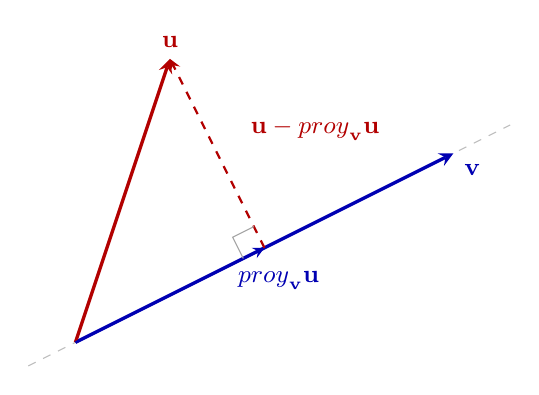
\begin{tikzpicture}[scale=1.2, >=stealth]
% Recta generada por v
\draw[gray!50, dashed] (-0.5,-0.25) -- (4.6,2.3);
% Vectores
\draw[->, blue!70!black, very thick] (0,0) -- (4,2) node[anchor=north west] {\small $\mathbf{v}$};
\draw[->, red!70!black, very thick] (0,0) -- (1,3) node[anchor=south] {\small $\mathbf{u}$};
\draw[->, blue!70!black, thick] (0,0) -- (2,1);
\node[blue!70!black, anchor=north] at (2.15,0.85) {\small $\operatorname{proy}_{\mathbf{v}}\mathbf{u}$};
% Componente ortogonal
\draw[->, red!70!black, thick, dashed] (2,1) -- (1,3);
\node[red!70!black, anchor=west] at (1.75,2.25) {\small $\mathbf{u}-\operatorname{proy}_{\mathbf{v}}\mathbf{u}$};
% Marca de ángulo recto en (2,1)
\draw[gray!70] (1.776,0.888) -- (1.664,1.112) -- (1.888,1.224);
\end{tikzpicture}
\caption{Proyección ortogonal de $\mathbf{u}$ sobre $\mathbf{v}$: el vector $\operatorname{proy}_{\mathbf{v}}\mathbf{u}$ vive en la recta generada por $\mathbf{v}$ y la diferencia $\mathbf{u}-\operatorname{proy}_{\mathbf{v}}\mathbf{u}$ es ortogonal a $\mathbf{v}$.}
\label{fig:proyeccion_ortogonal}
\end{figure}

\begin{theorem}[Expansión en base ortogonal]
Sea $S = \{ \mathbf{v}_1, \dots, \mathbf{v}_n \}$ una base ortogonal de $V$ (espacio vectorial con producto interno real). Para todo $\mathbf{u} \in V$ \(
\mathbf{u} = \sum_{i=1}^n \operatorname{proy}_{\mathbf{v}_i} \mathbf{u} = \sum_{i=1}^n \frac{\langle \mathbf{u}, \mathbf{v}_i \rangle}{\|\mathbf{v}_i\|^2} \mathbf{v}_i
\)
\begin{proof}
Como $S$ es base, existen escalares $k_1, \dots, k_n$ tales que: \(
\mathbf{u} = \sum_{j=1}^n k_j \mathbf{v}_j
\)

Para cada $i$, calculamos el producto interno con $\mathbf{v}_i$: \(
\langle \mathbf{u}, \mathbf{v}_i \rangle = \left\langle \sum_{j=1}^n k_j \mathbf{v}_j, \mathbf{v}_i \right\rangle = \sum_{j=1}^n k_j \langle \mathbf{v}_j, \mathbf{v}_i \rangle
\)

Por ortogonalidad ($\langle \mathbf{v}_j, \mathbf{v}_i \rangle = 0$ para $j \neq i$): \(
\langle \mathbf{u}, \mathbf{v}_i \rangle = k_i \langle \mathbf{v}_i, \mathbf{v}_i \rangle = k_i \|\mathbf{v}_i\|^2
\)


Despejando $k_i$: \(
k_i = \frac{\langle \mathbf{u}, \mathbf{v}_i \rangle}{\|\mathbf{v}_i\|^2}
\)


Sustituyendo en la combinación lineal:\(
\mathbf{u} = \sum_{i=1}^n \frac{\langle \mathbf{u}, \mathbf{v}_i \rangle}{\|\mathbf{v}_i\|^2} \mathbf{v}_i = \sum_{i=1}^n \operatorname{proy}_{\mathbf{v}_i} \mathbf{u}
\)
\end{proof}
\end{theorem}

\begin{theorem}[Descomposición ortogonal]
Sea $W$ subespacio de dimensión finita de $V$ (espacio vectorial con producto interno real). Para todo $\mathbf{u} \in V$, existen únicos $\mathbf{w} \in W$ y $\mathbf{w}^\perp \in W^\perp$ tales que:
\[
\mathbf{u} = \mathbf{w} + \mathbf{w}^\perp
\]
Además, $\mathbf{w} = \operatorname{proy}_W \mathbf{u}$ es la proyección ortogonal sobre $W$.
\end{theorem}

\begin{proof}
Sea $\{ \mathbf{v}_1, \dots, \mathbf{v}_k \}$ base ortogonal de $W$. Definimos: \(
\mathbf{w} = \sum_{i=1}^k \operatorname{proy}_{\mathbf{v}_i} \mathbf{u} = \sum_{i=1}^k \frac{\langle \mathbf{u}, \mathbf{v}_i \rangle}{\|\mathbf{v}_i\|^2} \mathbf{v}_i
\) 
y $\mathbf{w}^\perp = \mathbf{u} - \mathbf{w}$. Veamos que $\mathbf{w}^\perp \in W^\perp$. Para cada $\mathbf{v}_j$:
\begin{align*}
\langle \mathbf{w}^\perp, \mathbf{v}_j \rangle &= \langle \mathbf{u} - \mathbf{w}, \mathbf{v}_j \rangle \\
&= \langle \mathbf{u}, \mathbf{v}_j \rangle - \left\langle \sum_{i=1}^k \frac{\langle \mathbf{u}, \mathbf{v}_i \rangle}{\|\mathbf{v}_i\|^2} \mathbf{v}_i, \mathbf{v}_j \right\rangle \\
&= \langle \mathbf{u}, \mathbf{v}_j \rangle - \frac{\langle \mathbf{u}, \mathbf{v}_j \rangle}{\|\mathbf{v}_j\|^2} \langle \mathbf{v}_j, \mathbf{v}_j \rangle \\
&= \langle \mathbf{u}, \mathbf{v}_j \rangle - \langle \mathbf{u}, \mathbf{v}_j \rangle = 0
\end{align*}
Como los $\mathbf{v}_j$ generan $W$, $\mathbf{w}^\perp$ es ortogonal a todo $W$. La unicidad se sigue de que $W \cap W^\perp = \{\mathbf{0}\}$.
\end{proof}

\begin{theorem}\label{teodeo}
Sea $W$ subespacio de $V$ con base ortogonal $\{ \mathbf{v}_1, \dots, \mathbf{v}_r \}$. Para todo $\mathbf{u} \in V$, la proyección ortogonal sobre $W$ es: \(
\operatorname{proy}_W \mathbf{u} = \sum_{i=1}^r \operatorname{proy}_{\mathbf{v}_i} \mathbf{u}\)
\begin{proof}
Por el teorema de descomposición ortogonal, $\mathbf{u} = \mathbf{w} + \mathbf{w}^\perp$ con $\mathbf{w} \in W$ y $\mathbf{w}^\perp \in W^\perp$. Entonces:
\[
\operatorname{proy}_W \mathbf{u} = \mathbf{w} = \sum_{i=1}^r \frac{\langle \mathbf{w}, \mathbf{v}_i \rangle}{\|\mathbf{v}_i\|^2} \mathbf{v}_i
\]
Pero $\langle \mathbf{w}, \mathbf{v}_i \rangle = \langle \mathbf{u} - \mathbf{w}^\perp, \mathbf{v}_i \rangle = \langle \mathbf{u}, \mathbf{v}_i \rangle$ pues $\mathbf{w}^\perp \perp \mathbf{v}_i$. Así: \(
\operatorname{proy}_W \mathbf{u} = \sum_{i=1}^r \frac{\langle \mathbf{u}, \mathbf{v}_i \rangle}{\|\mathbf{v}_i\|^2} \mathbf{v}_i = \sum_{i=1}^r \operatorname{proy}_{\mathbf{v}_i} \mathbf{u}. \)
\end{proof}
\end{theorem}

\begin{theorem}[Proceso de Gram-Schmidt]\label{thm:cap07:gram-schmidt}
Todo espacio vectorial de dimensión finita con producto interno posee una base ortogonal.
\begin{proof}
Sea $\{ \mathbf{u}_1, \dots, \mathbf{u}_n \}$ base cualquiera de $V$. Construimos una base ortogonal $\{ \mathbf{v}_1, \dots, \mathbf{v}_n \}$ recursivamente:
\begin{align*}
\mathbf{v}_1 &= \mathbf{u}_1 \\
\mathbf{v}_2 &= \mathbf{u}_2 - \operatorname{proy}_{\mathbf{v}_1} \mathbf{u}_2 = \mathbf{u}_2 - \frac{\langle \mathbf{u}_2, \mathbf{v}_1 \rangle}{\|\mathbf{v}_1\|^2} \mathbf{v}_1 \\
\mathbf{v}_3 &= \mathbf{u}_3 - \operatorname{proy}_{\mathbf{v}_1} \mathbf{u}_3 - \operatorname{proy}_{\mathbf{v}_2} \mathbf{u}_3 \\
&\ \vdots \\
\mathbf{v}_k &= \mathbf{u}_k - \sum_{j=1}^{k-1} \operatorname{proy}_{\mathbf{v}_j} \mathbf{u}_k
\end{align*}
Cada $\mathbf{v}_k$ es ortogonal a $\mathbf{v}_1, \dots, \mathbf{v}_{k-1}$ por construcción, y el conjunto resultante es base ortogonal. Para obtener una base ortonormal se normaliza cada vector \(\mathbf{q}_i = \frac{\mathbf{v}_i}{\|\mathbf{v}_i\|}.\)
\end{proof}
\end{theorem}

\begin{figure}[H]
\centering
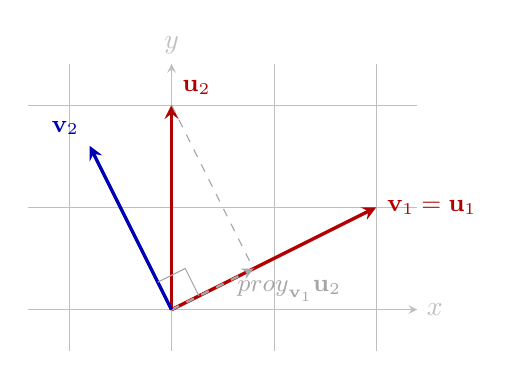
\begin{tikzpicture}[scale=1.3, >=stealth]
\draw[gray!50, very thin] (-1.4,-0.4) grid (2.4,2.4);
\draw[->, gray!50] (-1.4,0) -- (2.4,0) node[anchor=west] {$x$};
\draw[->, gray!50] (0,-0.4) -- (0,2.4) node[anchor=south] {$y$};
% Base original
\draw[->, red!70!black, very thick] (0,0) -- (2,1) node[anchor=west] {\small $\mathbf{v}_1=\mathbf{u}_1$};
\draw[->, red!70!black, very thick] (0,0) -- (0,2) node[anchor=south west] {\small $\mathbf{u}_2$};
% Proyección de u2 sobre v1
\draw[->, gray!70, thick, dashed] (0,0) -- (0.8,0.4);
\node[gray!70, anchor=north west] at (0.55,0.38) {\small $\operatorname{proy}_{\mathbf{v}_1}\mathbf{u}_2$};
\draw[dashed, gray!70] (0,2) -- (0.8,0.4);
% Vector ortogonalizado
\draw[->, blue!70!black, very thick] (0,0) -- (-0.8,1.6) node[anchor=south east] {\small $\mathbf{v}_2$};
% Marca de ángulo recto en el origen
\draw[gray!70] (0.268,0.134) -- (0.134,0.402) -- (-0.134,0.268);
\end{tikzpicture}
\caption{Proceso de Gram-Schmidt en $\mathbb{R}^2$: de la base $\{\mathbf{u}_1,\mathbf{u}_2\}$ se obtiene la base ortogonal $\{\mathbf{v}_1,\mathbf{v}_2\}$ tomando $\mathbf{v}_1=\mathbf{u}_1$ y restando de $\mathbf{u}_2$ su proyección sobre $\mathbf{v}_1$: $\mathbf{v}_2=\mathbf{u}_2-\operatorname{proy}_{\mathbf{v}_1}\mathbf{u}_2$.}
\label{fig:gram_schmidt_r2}
\end{figure}


\begin{example}[Extensión de un vector a una base ortogonal de $\mathbb{R}^3$]
Calcule una base ortogonal para $\mathbb{R}^3$ que contenga al vector ${\bf{v_1}}=(2,2,1).$
\begin{myproof}
\textbf{Paso 1. Estrategia.} Gram-Schmidt no construye bases de la nada: ortogonaliza una base dada respetando el orden. Por eso completamos $\mathbf{v_1}$ hasta una base cualquiera de $\mathbb{R}^3$ colocándolo \emph{primero}, y aplicamos el proceso; al no modificarse nunca el primer vector, $\mathbf{v_1}$ sobrevive en la base ortogonal final.

Tomamos la base inicial $\{\mathbf{v_1}, \mathbf{e_1}, \mathbf{e_2}\}$ con $\mathbf{e_1} = (1,0,0)$, $\mathbf{e_2} = (0,1,0)$, que es linealmente independiente porque $\det[\mathbf{v_1}\ \mathbf{e_1}\ \mathbf{e_2}] = 1 \neq 0$. Así $\mathbf{u_1} = \mathbf{v_1} = \begin{pmatrix} 2 \\ 2 \\ 1 \end{pmatrix}$, con $\|\mathbf{u_1}\|^2 = 9$.

\textbf{Paso 2. Ortogonalizar $\mathbf{e_1}$ contra $\mathbf{u_1}$.}
Proyección de $\mathbf{e_1}$ sobre $\mathbf{u_1}$:
\[
\operatorname{proy}_{\mathbf{u_1}} \mathbf{e_1} = \frac{2}{9} \begin{pmatrix} 2 \\ 2 \\ 1 \end{pmatrix} = \begin{pmatrix} \frac{4}{9} \\ \frac{4}{9} \\ \frac{2}{9} \end{pmatrix}
\]
\[
\mathbf{u_2} = \mathbf{e_1} - \operatorname{proy}_{\mathbf{u_1}} \mathbf{e_1} = \begin{pmatrix} 1 \\ 0 \\ 0 \end{pmatrix} - \begin{pmatrix} \frac{4}{9} \\ \frac{4}{9} \\ \frac{2}{9} \end{pmatrix} = \begin{pmatrix} \frac{5}{9} \\ -\frac{4}{9} \\ -\frac{2}{9} \end{pmatrix}
\]

\textbf{Paso 3. Ortogonalizar $\mathbf{e_2}$ contra $\mathbf{u_1}$ y $\mathbf{u_2}$.}
Proyección de $\mathbf{e_2}$ sobre $\mathbf{u_1}$:
\[
\operatorname{proy}_{\mathbf{u_1}} \mathbf{e_2} = \frac{2}{9} \begin{pmatrix} 2 \\ 2 \\ 1 \end{pmatrix} = \begin{pmatrix} \frac{4}{9} \\ \frac{4}{9} \\ \frac{2}{9} \end{pmatrix}
\]
Proyección de $\mathbf{e_2}$ sobre $\mathbf{u_2}$, con $\|\mathbf{u_2}\|^2 = \frac{5}{9}$ y $\mathbf{e_2} \cdot \mathbf{u_2} = -\frac{4}{9}$:
\[
\operatorname{proy}_{\mathbf{u_2}} \mathbf{e_2} = \frac{\mathbf{e_2} \cdot \mathbf{u_2}}{\mathbf{u_2} \cdot \mathbf{u_2}} \mathbf{u_2} = -\frac{4}{5} \begin{pmatrix} \frac{5}{9} \\ -\frac{4}{9} \\ -\frac{2}{9} \end{pmatrix} = \begin{pmatrix} -\frac{4}{9} \\ \frac{16}{45} \\ \frac{8}{45} \end{pmatrix}
\]
\[
\mathbf{u_3} = \mathbf{e_2} - \operatorname{proy}_{\mathbf{u_1}} \mathbf{e_2} - \operatorname{proy}_{\mathbf{u_2}} \mathbf{e_2} = \begin{pmatrix} 0 \\ 1 \\ 0 \end{pmatrix} - \begin{pmatrix} \frac{4}{9} \\ \frac{4}{9} \\ \frac{2}{9} \end{pmatrix} - \begin{pmatrix} -\frac{4}{9} \\ \frac{16}{45} \\ \frac{8}{45} \end{pmatrix} = \begin{pmatrix} 0 \\ \frac{1}{5} \\ -\frac{2}{5} \end{pmatrix}
\]

\textbf{Paso 4. Resultado.} Se verifica que los tres productos internos cruzados se anulan:
\[
\mathbf{u_1}\cdot\mathbf{u_2} = 0, \qquad \mathbf{u_1}\cdot\mathbf{u_3} = \tfrac{2}{5} - \tfrac{2}{5} = 0, \qquad \mathbf{u_2}\cdot\mathbf{u_3} = -\tfrac{4}{45} + \tfrac{4}{45} = 0,
\]
y como son tres vectores ortogonales no nulos en $\mathbb{R}^3$, forman una base que contiene a $\mathbf{v_1} = \mathbf{u_1}$:
\[
\boxed{\mathbf{u_1} = \begin{pmatrix} 2 \\ 2 \\ 1 \end{pmatrix}, \quad \mathbf{u_2} = \begin{pmatrix} \frac{5}{9} \\ -\frac{4}{9} \\ -\frac{2}{9} \end{pmatrix}, \quad \mathbf{u_3} = \begin{pmatrix} 0 \\ \frac{1}{5} \\ -\frac{2}{5} \end{pmatrix}}
\]
\end{myproof}
\end{example}


\begin{example}[Base ortonormal para $W \subseteq \mathbb{R}^3$ por Gram-Schmidt]
Sea $W = \operatorname{gen} \left\{ \begin{pmatrix} 1 \\ 1 \\ 1 \end{pmatrix}, \begin{pmatrix} 1 \\ 0 \\ -1 \end{pmatrix}, \begin{pmatrix} 2 \\ 0 \\ 3 \end{pmatrix} \right\}$. Hallar base ortonormal para $W$.
\begin{myproof}
\textbf{Paso 1. Aplicar Gram-Schmidt para obtener base ortogonal.} Con $\mathbf{u}_1 = (1,1,1)^T$, $\mathbf{u}_2 = (1,0,-1)^T$, $\mathbf{u}_3 = (2,0,3)^T$:
\begin{align*}
\mathbf{v}_1 &= \mathbf{u}_1 = \begin{pmatrix} 1 \\ 1 \\ 1 \end{pmatrix} \\
\mathbf{v}_2 &= \mathbf{u}_2 - \frac{\langle \mathbf{u}_2, \mathbf{v}_1 \rangle}{\|\mathbf{v}_1\|^2} \mathbf{v}_1 = \begin{pmatrix} 1 \\ 0 \\ -1 \end{pmatrix} - \frac{0}{3} \begin{pmatrix} 1 \\ 1 \\ 1 \end{pmatrix} = \begin{pmatrix} 1 \\ 0 \\ -1 \end{pmatrix} \\
\mathbf{v}_3 &= \mathbf{u}_3 - \frac{\langle \mathbf{u}_3, \mathbf{v}_1 \rangle}{\|\mathbf{v}_1\|^2} \mathbf{v}_1 - \frac{\langle \mathbf{u}_3, \mathbf{v}_2 \rangle}{\|\mathbf{v}_2\|^2} \mathbf{v}_2 \\
&= \begin{pmatrix} 2 \\ 0 \\ 3 \end{pmatrix} - \frac{5}{3} \begin{pmatrix} 1 \\ 1 \\ 1 \end{pmatrix} + \frac{1}{2} \begin{pmatrix} 1 \\ 0 \\ -1 \end{pmatrix} = \begin{pmatrix} \frac{5}{6} \\ -\frac{5}{3} \\ \frac{11}{6} \end{pmatrix}
\end{align*}

\textbf{Paso 2. Normalizar cada vector.}
\begin{align*}
\|\mathbf{v}_1\| &= \sqrt{3} \Rightarrow \mathbf{q}_1 = \tfrac{1}{\sqrt{3}} (1,1,1)^T \\
\|\mathbf{v}_2\| &= \sqrt{2} \Rightarrow \mathbf{q}_2 = \tfrac{1}{\sqrt{2}} (1,0,-1)^T \\
\|\mathbf{v}_3\| &= \tfrac{\sqrt{246}}{6} \Rightarrow \mathbf{q}_3 = \tfrac{6}{\sqrt{246}} \left(\tfrac{5}{6}, -\tfrac{5}{3}, \tfrac{11}{6}\right)^T
\end{align*}
$$\boxed{\left\{ \frac{1}{\sqrt{3}}\begin{pmatrix}1\\1\\1\end{pmatrix},\ \frac{1}{\sqrt{2}}\begin{pmatrix}1\\0\\-1\end{pmatrix},\ \frac{6}{\sqrt{246}}\begin{pmatrix}5/6\\-5/3\\11/6\end{pmatrix} \right\} \text{ es base ortonormal de } W.}$$
\end{myproof}
\end{example}


\begin{example}[Base ortogonal en $\mathcal{P}_2(\mathbb{R})$ por Gram-Schmidt]
Sea $B= \{1+x, x^2, x-x^2\}$, halle una base ortogonal para $B$ usando el producto interno $\langle p,q\rangle = \int_0^1 p(x)q(x)\,dx$.
\begin{myproof}
\textbf{Paso 1. Estrategia.} Aplicamos Gram-Schmidt a $B$ en el orden dado. El primer vector no se modifica, y cada uno de los siguientes se obtiene restándole sus proyecciones sobre los anteriores. Todos los productos internos son integrales sobre $[0,1]$, así que fijamos $\mathbf{v}_1 = 1+x$ y calculamos de una vez
\[
\langle \mathbf{v}_1, \mathbf{v}_1 \rangle = \int_0^1 (1+x)^2\,dx = \left[ x + x^2 + \frac{x^3}{3} \right]_0^1 = \frac{7}{3}.
\]

\textbf{Paso 2. Segundo vector.} Con $\langle x^2, \mathbf{v}_1\rangle = \int_0^1 x^2(1+x)\,dx = \frac{1}{3}+\frac{1}{4} = \frac{7}{12}$:
\begin{align*}
\mathbf{v}_2 &= x^2 - \frac{\langle x^2, \mathbf{v}_1\rangle}{\langle \mathbf{v}_1, \mathbf{v}_1\rangle} \mathbf{v}_1
    = x^2 - \frac{7/12}{7/3} (1+x) \\
    &= x^2 - \frac{1}{4}(1+x)
    = x^2 - \frac{1}{4}x - \frac{1}{4}
\end{align*}

\textbf{Paso 3. Tercer vector.} Necesitamos tres integrales más:
\[
\langle x-x^2, \mathbf{v}_1 \rangle = \frac{1}{4}, \qquad
\langle x-x^2, \mathbf{v}_2 \rangle = -\frac{1}{80}, \qquad
\langle \mathbf{v}_2, \mathbf{v}_2 \rangle = \frac{13}{240},
\]
de donde los coeficientes son $\frac{1/4}{7/3} = \frac{3}{28}$ y $\frac{-1/80}{13/240} = -\frac{3}{13}$. Entonces:
\begin{align*}
\mathbf{v}_3 &= (x - x^2) - \frac{\langle x - x^2, \mathbf{v}_1\rangle}{\langle \mathbf{v}_1, \mathbf{v}_1\rangle} \mathbf{v}_1 - \frac{\langle x - x^2, \mathbf{v}_2\rangle}{\langle \mathbf{v}_2, \mathbf{v}_2\rangle} \mathbf{v}_2 \\
    &= (x - x^2) - \frac{3}{28} (1+x) + \frac{3}{13} \left(x^2 - \frac{1}{4}x - \frac{1}{4}\right) \\
    &= \left(-x^2 + \frac{3}{13}x^2\right) + \left(x - \frac{3}{28}x - \frac{3}{52}x\right) + \left(-\frac{3}{28} - \frac{3}{52}\right) \\
    &= -\frac{10}{13}x^2 + \frac{76}{91}x - \frac{15}{91}
\end{align*}

\textbf{Paso 4. Resultado.} Se comprueba que $\langle \mathbf{v}_1, \mathbf{v}_2 \rangle = \langle \mathbf{v}_1, \mathbf{v}_3 \rangle = \langle \mathbf{v}_2, \mathbf{v}_3 \rangle = 0$, luego
$$\boxed{B_\perp = \left\{1+x,\; x^2 - \tfrac{1}{4}x - \tfrac{1}{4},\; -\tfrac{10}{13}x^2 + \tfrac{76}{91}x - \tfrac{15}{91}\right\}}$$
es una base ortogonal de $\mathcal{P}_2(\mathbb{R})$ para este producto interno.
\end{myproof}
\end{example}

\section{Proyección ortogonal y mínimos cuadrados}

\begin{definition}[Aproximación por mínimos cuadrados]
Sea $A \in \mathcal{M}_{m \times n}(\mathbb{R})$ y $b \in \mathbb{R}^m$. Si el sistema $Ax = b$ no tiene solución exacta (es decir, $b \notin \mathcal{C}(A)$), se busca $x$ tal que $Ax$ sea el vector más cercano posible a $b$, minimizando el error cuadrático: \(
\min_{x} \|b - Ax\|
.\) La mejor aproximación es el vector $Ax$ tal que $Ax = \operatorname{proy}_{\mathcal{C}(A)}(b)$.
\end{definition}

\begin{theorem}[Mejor aproximación]
Sea $W$ subespacio de $V$ (espacio vectorial con producto interno real, dimensión finita) y $b \in V$. La proyección ortogonal $\operatorname{proy}_W(b)$ es el único vector en $W$ que minimiza la distancia a $b$:
\[
\|b - \operatorname{proy}_W(b)\| \leq \|b - w\| \quad \forall w \in W
\]
\begin{proof}
Por descomposición ortogonal, $b = \operatorname{proy}_W(b) + r$ con $r \perp W$. Para cualquier $w \in W$:
\[
b - w = (b - \operatorname{proy}_W(b)) + (\operatorname{proy}_W(b) - w)
\]
Como $r \perp (\operatorname{proy}_W(b) - w)$:
\[
\|b - w\|^2 = \|r\|^2 + \|\operatorname{proy}_W(b) - w\|^2 \geq \|r\|^2
\]
La igualdad se da solo cuando $w = \operatorname{proy}_W(b)$.
\end{proof}
\end{theorem}

\begin{theorem}[Ecuaciones normales]
Dado $A \in \mathbb{R}^{m \times n}$ y $b \in \mathbb{R}^m$, el vector $x$ que minimiza $\|b - Ax\|$ satisface:
\[
A^T A x = A^T b
\]
\begin{proof}
El residuo $r = b - Ax$ debe ser ortogonal a $\mathcal{C}(A)$, es decir:
\[
A^T r = 0 \implies A^T(b - Ax) = 0 \implies A^T A x = A^T b
\]
\end{proof}
\end{theorem}

\begin{example}[Solución por mínimos cuadrados — sistema $3\times 3$]
Resuelve por mínimos cuadrados:
\[
\begin{cases}
3x + 5y + 9z = 1 \\
7x + 8y + 4z = 1 \\
x + z = 4
\end{cases}
\]
\begin{myproof}
Matriz del sistema y vector independiente:
\[
A = \begin{pmatrix}
3 & 5 & 9 \\
7 & 8 & 4 \\
1 & 0 & 1
\end{pmatrix}, \quad
b = \begin{pmatrix} 1 \\ 1 \\ 4 \end{pmatrix}
\]

\textbf{Paso 1. Cálculo de $A^T A$}
\[
A^T A = \begin{pmatrix}
3 & 7 & 1 \\
5 & 8 & 0 \\
9 & 4 & 1
\end{pmatrix}
\begin{pmatrix}
3 & 5 & 9 \\
7 & 8 & 4 \\
1 & 0 & 1
\end{pmatrix}
= \begin{pmatrix}
59 & 71 & 56 \\
71 & 89 & 77 \\
56 & 77 & 98
\end{pmatrix}
\]

\textbf{Paso 2. Cálculo de $A^T b$}
\[
A^T b = \begin{pmatrix}
3 & 7 & 1 \\
5 & 8 & 0 \\
9 & 4 & 1
\end{pmatrix}
\begin{pmatrix} 1 \\ 1 \\ 4 \end{pmatrix}
= \begin{pmatrix} 14 \\ 13 \\ 17 \end{pmatrix}
\]

\textbf{Paso 3. Resolución del sistema}
\[
\begin{pmatrix}
59 & 71 & 56 \\
71 & 89 & 77 \\
56 & 77 & 98
\end{pmatrix}
\begin{pmatrix} x \\ y \\ z \end{pmatrix}
= \begin{pmatrix} 14 \\ 13 \\ 17 \end{pmatrix}
\]
Solución exacta (el sistema es consistente):
\[
x = \left( \frac{205}{63},\ -\frac{65}{21},\ \frac{47}{63} \right)
\]

\textbf{Verificación:}
\begin{align*}
3\left(\frac{205}{63}\right) + 5\left(-\frac{65}{21}\right) + 9\left(\frac{47}{63}\right) &= 1 \\
7\left(\frac{205}{63}\right) + 8\left(-\frac{65}{21}\right) + 4\left(\frac{47}{63}\right) &= 1 \\
\frac{205}{63} + \frac{47}{63} &= 4
\end{align*}
Residuo: $\|b - Ax\| = 0$
$$\boxed{x = \left(\tfrac{205}{63},\ -\tfrac{65}{21},\ \tfrac{47}{63}\right),\quad \|b - Ax\| = 0\ \text{(solución exacta).}}$$
\end{myproof}
\end{example}

\begin{example}[Solución por mínimos cuadrados — sistema $4\times 3$]
Resuelve por mínimos cuadrados:
\[
\begin{pmatrix}
2 & -1 & 0 \\
3 & 1 & 2 \\
-1 & 4 & 5 \\
1 & 2 & 4
\end{pmatrix}
X =
\begin{pmatrix} -1 \\ 0 \\ 1 \\ 2 \end{pmatrix}
\]
\begin{myproof}
\textbf{Paso 1. Cálculo de $A^T A$ y $A^T b$.}
\[
A^T A = \begin{pmatrix}
15 & -1 & 5 \\
-1 & 22 & 30 \\
5 & 30 & 45
\end{pmatrix}, \quad
A^T b = \begin{pmatrix} -1 \\ 9 \\ 13 \end{pmatrix}
\]

\textbf{Paso 2. Solución del sistema normal.}
\[
X = \left( -\dfrac{31}{91},\ -\dfrac{4}{7},\ \dfrac{46}{65} \right)
\]

\textbf{Paso 3. Error residual.}
\[
\|b - AX\| = \sqrt{\frac{7969}{5915}} \approx 1.162
\]
$$\boxed{X = \left(-\dfrac{31}{91},\ -\dfrac{4}{7},\ \dfrac{46}{65}\right),\quad \|b - AX\| \approx 1.162.}$$
\end{myproof}
\end{example}

\begin{theorem}[Solución única]
Si las columnas de $A$ son linealmente independientes, entonces:
\begin{enumerate}
    \item $A^T A$ es invertible
    \item La solución única es $x = (A^T A)^{-1} A^T b$
    \item Con descomposición QR $A = QR$, $x = R^{-1} Q^T b$
\end{enumerate}
\end{theorem}

\begin{example}[Ley de Hooke: estimación de la constante de un resorte]
La ley de Hooke en física determina que la longitud $x$ en un resorte uniforme es una función lineal de la fuerza $y$ aplicada. Si se expresa esta relación como $y=mx+b,$ entonces el coeficiente $m$ es llamado la constante del resorte.

\begin{table}[H]
\centering
\begin{tabular}{|c|l|l|l|l|}
\hline
Peso (y) kg  & 1.5   & 2.7   & 4.9  & 6.7    \\ \hline
Longitud (x) m & 6.1 & 7.6 & 8.7 & 10.4 \\ \hline
\end{tabular}
\caption{Datos de estiramiento del resorte}
\end{table}  

\begin{enumerate}[$(a)$]
\item Encuentre la recta de ajuste por mínimos cuadrados de los siguientes datos y úselos para estimar la constante del resorte involucrado.
\item Grafique la recta los puntos.
\end{enumerate}

\begin{myproof}
\textbf{Paso 1. Estrategia.} Los cuatro datos exigen que la recta $y = mx + b$ pase por cuatro puntos, lo que da un sistema de cuatro ecuaciones con dos incógnitas: sobredeterminado y, salvo coincidencia, inconsistente. En lugar de una solución exacta buscamos la que minimiza $\|\mathbf{b} - A\mathbf{x}\|$, es decir, la solución de las ecuaciones normales $A^TA\mathbf{x} = A^T\mathbf{b}$. La pendiente $m$ de esa recta es la constante del resorte.

\textbf{Paso 2. Plantear las ecuaciones normales (parte $a$).} Definimos
\begin{itemize}
\item vector de observaciones: \(\mathbf{b} = \begin{pmatrix} 1.5 \\ 2.7 \\ 4.9 \\ 6.7 \end{pmatrix}\)
\item matriz de diseño: \(A = \begin{pmatrix} 1 & 6.1 \\ 1 & 7.6 \\ 1 & 8.7 \\ 1 & 10.4 \end{pmatrix}\)
\item vector de parámetros: \(\mathbf{x} = \begin{pmatrix} b \\ m \end{pmatrix}\)
\end{itemize}

Entonces:

\[
A^TA = \begin{pmatrix}
1 & 1 & 1 & 1 \\
6.1 & 7.6 & 8.7 & 10.4
\end{pmatrix}
\begin{pmatrix}
1 & 6.1 \\
1 & 7.6 \\
1 & 8.7 \\
1 & 10.4
\end{pmatrix} = \begin{pmatrix}
4 & 32.8 \\
32.8 & 278.82
\end{pmatrix}
\]

\[
A^T\mathbf{b} = \begin{pmatrix}
1 & 1 & 1 & 1 \\
6.1 & 7.6 & 8.7 & 10.4
\end{pmatrix}
\begin{pmatrix}
1.5 \\ 2.7 \\ 4.9 \\ 6.7
\end{pmatrix} = \begin{pmatrix}
15.8 \\ 141.98
\end{pmatrix}
\]

\textbf{Paso 3. Resolver el sistema normal (parte $a$).} El sistema es
\[
\begin{pmatrix}
4 & 32.8 \\
32.8 & 278.82
\end{pmatrix}
\begin{pmatrix}
b \\ m
\end{pmatrix} =
\begin{pmatrix}
15.8 \\ 141.98
\end{pmatrix}
\]

Calculamos el determinante:
\[
\det(A^TA) = (4)(278.82) - (32.8)(32.8) = 1115.28 - 1075.84 = 39.44
\]

Como $\det(A^TA) \neq 0$, el sistema normal tiene solución única y la obtenemos por la regla de Cramer:
\[
b = \frac{
\begin{vmatrix}
15.8 & 32.8 \\
141.98 & 278.82
\end{vmatrix}
}{\det(A^TA)} = \frac{(15.8)(278.82) - (32.8)(141.98)}{39.44} = \frac{4405.356 - 4657.344}{39.44} = \frac{-251.988}{39.44} \approx -6.389
\]

\[
m = \frac{
\begin{vmatrix}
4 & 15.8 \\
32.8 & 141.98
\end{vmatrix}
}{\det(A^TA)} = \frac{(4)(141.98) - (32.8)(15.8)}{39.44} = \frac{567.92 - 518.24}{39.44} = \frac{49.68}{39.44} \approx 1.2597
\]

\textbf{Paso 4. Resultado y gráfica (parte $b$).} La recta de mínimos cuadrados y la constante del resorte son
\[
\boxed{y = 1.2597x - 6.389, \qquad m \approx 1.2597\ \text{kg/m}}
\]
La figura confirma el ajuste: los cuatro puntos experimentales quedan repartidos a ambos lados de la recta, como corresponde a un residuo de norma mínima.

\begin{figure}[H]
\centering
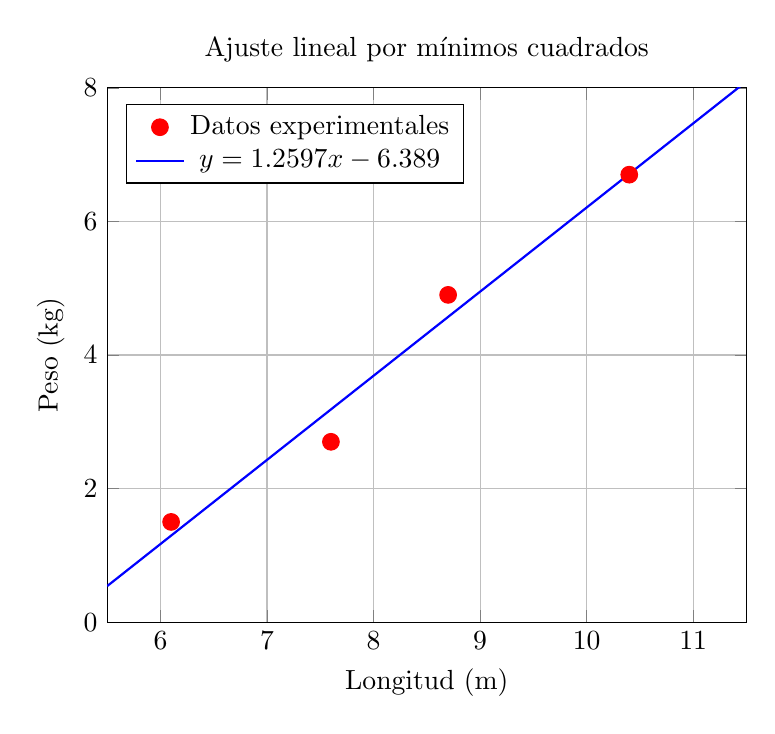
\begin{tikzpicture}
\begin{axis}[
    title={Ajuste lineal por mínimos cuadrados},
    xlabel={Longitud (m)},
    ylabel={Peso (kg)},
    grid=both,
    xmin=5.5, xmax=11.5,
    ymin=0, ymax=8,
    legend pos=north west,
    scaled ticks=false,
    width=0.8\textwidth
]
\addplot[only marks, mark=*, red, mark size=3pt] coordinates {
    (6.1,1.5)
    (7.6,2.7)
    (8.7,4.9)
    (10.4,6.7)
};
\addlegendentry{Datos experimentales}
\addplot[domain=5.5:11.5, blue, thick, samples=2] {1.2597*x - 6.389};
\addlegendentry{$y = 1.2597x - 6.389$}
\end{axis}
\end{tikzpicture}
\caption{Recta de mínimos cuadrados para los datos del resorte}
\label{fig:recta_minimos_cuadrados}
\end{figure}
\end{myproof}
\end{example}


\begin{rem}[Regresión polinómica]\label{rem:regresion_polinomica}
El método de mínimos cuadrados no se limita a rectas. Para ajustar puntos $\{(x_i,y_i)\}_{i=1}^n$ al polinomio $y = \sum_{k=0}^m a_k x^k$, construimos:
\[
M = \begin{pmatrix}
1 & x_1 & \cdots & x_1^m \\
\vdots & \vdots & \ddots & \vdots \\
1 & x_n & \cdots & x_n^m
\end{pmatrix}, \quad
V = \begin{pmatrix} a_0 \\ \vdots \\ a_m \end{pmatrix}, \quad
Y = \begin{pmatrix} y_1 \\ \vdots \\ y_n \end{pmatrix}
\]
Solución por mínimos cuadrados:
\[
V = (M^T M)^{-1} M^T Y
\]
La matriz $M$ es la matriz de Vandermonde de los nodos $x_i$; cuando los $x_i$ son distintos y $n > m$, $M^T M$ es invertible y el ajuste es único.
\end{rem}

\section{Series de Fourier}

\begin{definition}[Serie de Fourier]
Para $f$ periódica en $[0, 2\pi]$, con producto interno $\langle f, g \rangle = \int_0^{2\pi} f(x) g(x)  dx$:
\[
f(x) \approx a_0 + \sum_{k=1}^n (a_k \cos kx + b_k \sin kx)
\]
donde:
\begin{align*}
a_0 &= \frac{1}{2\pi} \int_0^{2\pi} f(x)  dx \\
a_k &= \frac{1}{\pi} \int_0^{2\pi} f(x) \cos kx  dx \\
b_k &= \frac{1}{\pi} \int_0^{2\pi} f(x) \sin kx  dx
\end{align*}
\end{definition}

\begin{example}[{Series de Fourier en $[0,2\pi]$}]
Calcule la serie de Fourier correspondiente para las siguientes funciones en el intervalo $\left[ 0,2\pi \right]$:
\begin{enumerate}[$a)$]
\item $f(x)=x.$
\item $f(x)=8.$
\item $f(x)=x^2+2x+1.$
\end{enumerate}
\begin{myproof}
\textbf{Paso 1. Estrategia.} Las tres funciones son polinomios, así que basta aplicar las fórmulas de la definición. Como todos los integrandos se reducen a combinaciones de $x^j\cos kx$ y $x^j\sin kx$ con $j \leq 2$, calculamos una vez por partes las integrales auxiliares sobre $[0,2\pi]$, válidas para todo entero $k \geq 1$:
\[
\int_0^{2\pi}\! \cos kx\,dx = \int_0^{2\pi}\! \sin kx\,dx = 0, \qquad
\int_0^{2\pi}\! x\cos kx\,dx = 0, \qquad
\int_0^{2\pi}\! x\sin kx\,dx = -\frac{2\pi}{k},
\]
\[
\int_0^{2\pi}\! x^2\cos kx\,dx = \frac{4\pi}{k^2}, \qquad
\int_0^{2\pi}\! x^2\sin kx\,dx = -\frac{4\pi^2}{k}.
\]
Conviene subrayar que el intervalo es $[0,2\pi]$ y no $[-\pi,\pi]$: aquí no hay simetría par ni impar que anule coeficientes, y en particular no aparecen factores $(-1)^k$.

\textbf{Paso 2. Parte $a)$: $f(x)=x$.}
\[
a_0 = \frac{1}{2\pi}\int_0^{2\pi}\! x\,dx = \frac{1}{2\pi}\cdot 2\pi^2 = \pi, \qquad
a_k = \frac{1}{\pi}\cdot 0 = 0, \qquad
b_k = \frac{1}{\pi}\left(-\frac{2\pi}{k}\right) = -\frac{2}{k}.
\]
\[
f(x) \sim \pi - 2 \sum_{k=1}^{\infty} \frac{\sin(kx)}{k}
\]

\textbf{Paso 3. Parte $b)$: $f(x)=8$.} Al ser constante, $a_0 = \frac{1}{2\pi}\cdot 8 \cdot 2\pi = 8$, mientras que $a_k$ y $b_k$ son múltiplos de $\int_0^{2\pi}\cos kx\,dx$ y $\int_0^{2\pi}\sin kx\,dx$, ambas nulas. Luego $a_k = b_k = 0$ y la serie se reduce a su término constante:
\[
f(x) \sim 8
\]

\textbf{Paso 4. Parte $c)$ y resultado.} Para $f(x)=x^2+2x+1$ usamos linealidad de la integral y las fórmulas del Paso 1:
\begin{align*}
a_0 &= \frac{1}{2\pi}\left( \frac{8\pi^3}{3} + 4\pi^2 + 2\pi \right) = \frac{4\pi^2}{3} + 2\pi + 1, \\
a_k &= \frac{1}{\pi}\left( \frac{4\pi}{k^2} + 2\cdot 0 + 0 \right) = \frac{4}{k^2}, \\
b_k &= \frac{1}{\pi}\left( -\frac{4\pi^2}{k} + 2\left(-\frac{2\pi}{k}\right) + 0 \right) = -\frac{4(\pi+1)}{k}.
\end{align*}
Reuniendo las tres series:
\[
\boxed{
\begin{aligned}
a)\ & f(x) \sim \pi - 2 \sum_{k=1}^{\infty} \frac{\sin(kx)}{k} \\
b)\ & f(x) \sim 8 \\
c)\ & f(x) \sim \left( \frac{4\pi^2}{3} + 2\pi + 1 \right) + \sum_{k=1}^{\infty} \left[ \frac{4}{k^2} \cos(kx) - \frac{4(\pi+1)}{k} \sin(kx) \right]
\end{aligned}
}
\]
\end{myproof}
\end{example}

\begin{lemma}[Polinomio de Taylor]
Si $f$ es analítica en $x=a$:
\[
f(x) = \sum_{j=0}^\infty \frac{f^{(j)}(a)}{j!} (x - a)^j
\]
\begin{proof}
Desarrollo en serie de potencias alrededor de $x=a$ con coeficientes $a_j = f^{(j)}(a)/j!$.
\end{proof}
\end{lemma}

\begin{theorem}[Fórmula de Euler]\label{demformeuler}
Para $\theta \in \mathbb{R}$:
\[
e^{i\theta} = \cos \theta + i \sin \theta
\]
\begin{proof}
Por series de Taylor:
\begin{align*}
e^{ix} &= \sum_{k=0}^\infty \frac{(ix)^k}{k!} \\
\cos x &= \sum_{k=0}^\infty \frac{(-1)^k x^{2k}}{(2k)!} \\
\sin x &= \sum_{k=0}^\infty \frac{(-1)^k x^{2k+1}}{(2k+1)!}
\end{align*}
Se verifica $e^{ix} = \cos x + i \sin x$.
\end{proof}
\end{theorem}


\section{Problemas resueltos adicionales}

% Intermedio
\begin{prob}
Sea $A=\left( \begin{array}{ccc} 
	1&0&1\\
	0&1&0\\
	\end{array} \right).$ 
	
	\begin{enumerate} 
	\item Encuentre una base ortonormal para el espacio fila de $A.$
	\item Encuentre el rango y la nulidad de $A.$
    \item Encuentre una base para el complemento ortogonal del espacio fila de $A.$
	\end{enumerate}	
\begin{myproof}
\textbf{Paso 1. (a)} Las filas de \( A \) son \( \mathbf{r}_1 = (1,0,1) \) y \( \mathbf{r}_2 = (0,1,0) \). Son ortogonales: \( \langle \mathbf{r}_1, \mathbf{r}_2 \rangle = 0 \), así que basta normalizar. Normas: \( \|\mathbf{r}_1\| = \sqrt{2} \), \( \|\mathbf{r}_2\| = 1 \). Base ortonormal:
\[
\boxed{\mathbf{q}_1 = \frac{1}{\sqrt{2}} (1, 0, 1), \quad \mathbf{q}_2 = (0, 1, 0)}
\]

\textbf{Paso 2. (b)} Las filas son linealmente independientes, así que \( \text{rango}(A) = 2 \); por el teorema de rango-nulidad, \( \text{nulidad}(A) = 3 - 2 = 1 \).
\[
\boxed{\text{rango}(A) = 2, \quad \text{nulidad}(A) = 1}
\]

\textbf{Paso 3. (c)} El complemento ortogonal del espacio fila es el espacio nulo de \( A \). Resolviendo \( A\mathbf{x} = \mathbf{0} \):
\[
\begin{cases}
x_1 + x_3 = 0 \\
x_2 = 0
\end{cases} \implies \mathbf{x} = t \begin{pmatrix} -1 \\ 0 \\ 1 \end{pmatrix}.
\]
Base: \( \boxed{\left\{ \begin{pmatrix} -1 \\ 0 \\ 1 \end{pmatrix} \right\}} \).
\end{myproof}
\end{prob}

% ------------------ PROBLEMA 2 ------------------
% Intermedio
\begin{prob}
Una altura de un triángulo es cada uno de los segmentos que une un vértice con un punto de su lado opuesto o de su prolongación y es perpendicular a dicho lado.
\begin{figure}[H]
\centering
\begin{tikzpicture}[scale=0.7, rotate=-20]
\coordinate (A) at (0,0);
\coordinate (B) at (5,3);
\coordinate (C) at (1,4);
\draw[thick] (A) -- (B) -- (C) -- cycle;
\coordinate (D) at ($(A)!(B)!(C)$);
\draw[thick, red] (B) -- (D);
\draw[thick] (D) -- ++(0.3,0.15) -- ++(-0.15,0.3) -- ++(-0.3,-0.15);
\node[below left] at (A) {$A$};
\node[above right] at (B) {$B$};
\node[above left] at (C) {$C$};
\node[below right] at (D) {$D$};
\end{tikzpicture}
\caption{Altura de un triángulo}\label{fig:altura_triangulo}
\end{figure}
\begin{enumerate}
\item Sea $V$ un espacio vectorial con producto interno. Suponga que $\mathbf{u},$ $\mathbf{v},$ y $\mathbf{w}$ son vectores en $V$ que forman un triángulo como se muestra en la figura \ref{fig:altura_triangulo}. Calcule en términos de $\mathbf{u},$ $\mathbf{v}$ y $\mathbf{w}$ la altura $\mathbf{h}$ bajada desde $B$ al lado opuesto.
\item Dado el triángulo con vértices $A=(8,7,11),$ $B=(11,17,22)$ y $C=(5,3,11)$ use el producto interno usual de $\mathbb{R}^3$ para calcular las ecuaciones simétricas de la altura bajada desde el vértice $B$ al lado opuesto.
\end{enumerate}
\begin{myproof}
\textbf{Paso 1. (a)} Sean \( \overrightarrow{AB} = \mathbf{u} \), \( \overrightarrow{AC} = \mathbf{v} \), \( \overrightarrow{BC} = \mathbf{w} \). La proyección ortogonal de \( \overrightarrow{AB} \) sobre \( \overrightarrow{AC} \) es:
\[
\operatorname{proy}_{\mathbf{v}} \mathbf{u} = \frac{\langle \mathbf{u}, \mathbf{v} \rangle}{\|\mathbf{v}\|^2} \mathbf{v}.
\]
La altura es la componente de $\mathbf{u}$ perpendicular a $\mathbf{v}$:
\[
\boxed{\mathbf{h} = \mathbf{u} - \operatorname{proy}_{\mathbf{v}} \mathbf{u}}
\]

\textbf{Paso 2. (b)} Calculamos los vectores \( \overrightarrow{BA} = (-3, -10, -11) \) y \( \overrightarrow{AC} = (-3, -4, 0) \), y la proyección de \( \overrightarrow{BA} \) sobre \( \overrightarrow{AC} \):
\[
\operatorname{proy}_{\overrightarrow{AC}}(\overrightarrow{BA}) = \frac{\langle (-3,-10,-11), (-3,-4,0) \rangle}{\|(-3,-4,0)\|^2} (-3,-4,0) = \frac{9+40}{25}(-3,-4,0) = \frac{49}{25}(-3,-4,0).
\]

\textbf{Paso 3.} Vector altura:
\[
\mathbf{h} = \overrightarrow{BA} - \operatorname{proy} = \left(\frac{72}{25}, -\frac{54}{25}, -11\right).
\]
Escalando por 25, la dirección es $(72,-54,-275)$. Ecuaciones simétricas de la recta que pasa por \(B=(11,17,22)\) con dirección \(\mathbf{h}\):
\[
\boxed{\frac{x-11}{72} = \frac{y-17}{-54} = \frac{z-22}{-275}}.
\]
\end{myproof}
\end{prob}

% Intermedio
\begin{prob}
Calcule la serie de Fourier para la función $f(x)=9x^2+4x$ en el intervalo $\left[0,2\pi\right].$
\begin{myproof}
\textbf{Paso 1. Coeficiente $a_0$.} Con $\int_0^{2\pi} x\,dx = 2\pi^2$ y $\int_0^{2\pi} x^2\,dx = \frac{8\pi^3}{3}$:
\[
a_0 = \frac{1}{2\pi}\int_0^{2\pi} (9x^2+4x)\,dx = \frac{1}{2\pi}\left(9\cdot\frac{8\pi^3}{3} + 4\cdot 2\pi^2\right) = 12\pi^2 + 4\pi.
\]

\textbf{Paso 2. Coeficientes $a_k$.} Con $\int_0^{2\pi} x\cos kx\,dx = 0$ y $\int_0^{2\pi} x^2\cos kx\,dx = \frac{4\pi}{k^2}$:
\[
a_k = \frac{1}{\pi}\left(9\cdot\frac{4\pi}{k^2} + 4\cdot 0\right) = \frac{36}{k^2}.
\]

\textbf{Paso 3. Coeficientes $b_k$.} Con $\int_0^{2\pi} x\sin kx\,dx = -\frac{2\pi}{k}$ y $\int_0^{2\pi} x^2\sin kx\,dx = -\frac{4\pi^2}{k}$:
\[
b_k = \frac{1}{\pi}\left(9\left(-\frac{4\pi^2}{k}\right) + 4\left(-\frac{2\pi}{k}\right)\right) = -\frac{36\pi + 8}{k}.
\]

\textbf{Paso 4. Serie.}
\[
\boxed{f(x) \sim (12\pi^2 + 4\pi) + \sum_{k=1}^{\infty} \left[ \frac{36}{k^2} \cos(kx) - \frac{36\pi + 8}{k} \sin(kx) \right]}
\]
\end{myproof}
\end{prob}

% Intermedio
\begin{prob}
Sea $A=\left( \begin{array}{cccc} 
	1&0&1&1\\
	0&1&1&0\\
	0&1&0&1\\
	\end{array} \right).$ 
	\begin{enumerate}
	\item Encuentre una base ortonormal para el espacio fila de $A.$ Determine el rango y la nulidad de $A.$
	\item Encuentre una base para el complemento ortogonal del espacio fila de $A.$
	\end{enumerate}
\begin{myproof}
\textbf{Paso 1. (a)} Filas de \( A \): \( \mathbf{r}_1 = (1,0,1,1) \), \( \mathbf{r}_2 = (0,1,1,0) \), \( \mathbf{r}_3 = (0,1,0,1) \).
Aplicamos Gram-Schmidt para obtener una base ortogonal:
\begin{align*}
\mathbf{v}_1 &= \mathbf{r}_1 = (1,0,1,1), \\
\mathbf{v}_2 &= \mathbf{r}_2 - \frac{\langle \mathbf{r}_2, \mathbf{v}_1 \rangle}{\|\mathbf{v}_1\|^2} \mathbf{v}_1
= (0,1,1,0) - \frac{1}{3}(1,0,1,1) = \left(-\frac{1}{3},1,\frac{2}{3},-\frac{1}{3}\right), \\
\mathbf{v}_3 &= \mathbf{r}_3 - \frac{\langle \mathbf{r}_3, \mathbf{v}_1 \rangle}{\|\mathbf{v}_1\|^2} \mathbf{v}_1 - \frac{\langle \mathbf{r}_3, \mathbf{v}_2 \rangle}{\|\mathbf{v}_2\|^2} \mathbf{v}_2 \\
&= (0,1,0,1) - \frac{1}{3}(1,0,1,1) - \frac{\langle (0,1,0,1), (-\frac{1}{3},1,\frac{2}{3},-\frac{1}{3}) \rangle}{\|(-\frac{1}{3},1,\frac{2}{3},-\frac{1}{3})\|^2} \left(-\frac{1}{3},1,\frac{2}{3},-\frac{1}{3}\right) \\
&= (0,1,0,1) - \frac{1}{3}(1,0,1,1) - \frac{\frac{2}{3}}{\frac{5}{3}} \left(-\frac{1}{3},1,\frac{2}{3},-\frac{1}{3}\right) \\
&= (0,1,0,1) - \frac{1}{3}(1,0,1,1) - \frac{2}{5} \left(-\frac{1}{3},1,\frac{2}{3},-\frac{1}{3}\right) \\
&= \left(-\frac{1}{3}, 1, -\frac{1}{3}, \frac{2}{3}\right) - \frac{2}{5}\left(-\frac{1}{3},1,\frac{2}{3},-\frac{1}{3}\right) \\
&= \left(-\frac{1}{3}+\frac{2}{15}, 1-\frac{2}{5}, -\frac{1}{3}-\frac{4}{15}, \frac{2}{3}+\frac{2}{15}\right) \\
&= \left(-\frac{1}{5}, \frac{3}{5}, -\frac{3}{5}, \frac{4}{5}\right).
\end{align*}
\textbf{Paso 2.} Normalizando:
\[
\|\mathbf{v}_1\| = \sqrt{3},\quad \|\mathbf{v}_2\| = \sqrt{\frac{5}{3}},\quad \|\mathbf{v}_3\| = \sqrt{\frac{35}{25}} = \frac{\sqrt{35}}{5}.
\]
Base ortonormal:
\[
\boxed{
\mathbf{q}_1 = \frac{1}{\sqrt{3}}(1,0,1,1),\quad
\mathbf{q}_2 = \sqrt{\frac{3}{5}}\left(-\frac{1}{3},1,\frac{2}{3},-\frac{1}{3}\right),\quad
\mathbf{q}_3 = \frac{5}{\sqrt{35}}\left(-\frac{1}{5},\frac{3}{5},-\frac{3}{5},\frac{4}{5}\right)
}
\]
\textbf{Paso 3.} Las filas son linealmente independientes, así que rango \( = 3 \). Por el teorema de rango-nulidad, nulidad \( = 4-3 = 1 \).
\[
\boxed{\text{rango}(A) = 3, \quad \text{nulidad}(A) = 1}
\]

\textbf{Paso 4. (b)} El complemento ortogonal del espacio fila es el espacio nulo de \( A \). Resolviendo \( A\mathbf{x} = 0 \):
\[
\begin{cases}
x_1 + x_3 + x_4 = 0 \\
x_2 + x_3 = 0 \\
x_2 + x_4 = 0
\end{cases}
\Rightarrow x_2 = -x_3,\; x_4 = x_3,\; x_1 = -x_3 - x_4 = -2x_3.
\]
Por tanto, \( \mathbf{x} = t(-2,-1,1,1) \). Base:
\[
\boxed{\{(-2,-1,1,1)\}}.
\]
\end{myproof}
\end{prob}


% Desafiante
\begin{prob}
Sea $V=\mathcal{P}_{2}(\mathbb{R})$. Dados dos vectores $\mathbf{p}=a_0+a_1x+a_2x^2$ y  $\mathbf{q}=b_0+b_1x+b_2x^2$  defina el producto interno en $V$ como $\left\langle \mathbf{p},\mathbf{q} \right\rangle=a_0b_0+a_1b_1+a_2b_2$. 

Si $H=\text{gen}\lbrace \mathbf{p_1}=1+2x^2,\mathbf{p_2}=2+x+x^2\rbrace$ 
\begin{enumerate}
\item Calcule una base para $H^{\perp}$.
\item Calcule una base ortogonal para $H$.
\item Sea $\mathbf{q}=2+5x+9x^2$. Calcule $\text{proy}_{H}\mathbf{q}$.
\item Calcule la distancia mínima de $\mathbf{q}$ al subespacio $H$.
\end{enumerate}
\begin{myproof}
\textbf{Paso 1. (a)} \( H^\perp = \{ p \in V : \langle p, h \rangle = 0 \ \forall h \in H \} \).
Resolviendo:
\[
\langle a_0 + a_1x + a_2x^2, 1 + 2x^2 \rangle = a_0 + 2a_2 = 0,
\]
\[
\langle a_0 + a_1x + a_2x^2, 2 + x + x^2 \rangle = 2a_0 + a_1 + a_2 = 0.
\]
De la primera, \( a_0 = -2a_2 \). Sustituyendo: \( -4a_2 + a_1 + a_2 = 0 \Rightarrow a_1 = 3a_2 \).
Por tanto, \( p = a_2(-2 + 3x + x^2) \). Base:
\[
\boxed{\{-2 + 3x + x^2\}}.
\]

\textbf{Paso 2. (b)} Aplicamos Gram-Schmidt a \( h_1 = 1+2x^2 \), \( h_2 = 2+x+x^2 \):
\[
v_1 = h_1 = 1+2x^2.
\]
\[
v_2 = h_2 - \frac{\langle h_2, v_1 \rangle}{\langle v_1, v_1 \rangle} v_1
= (2+x+x^2) - \frac{4}{5}(1+2x^2)
= 2+x+x^2 - \frac{4}{5} - \frac{8}{5}x^2
= \frac{6}{5} + x - \frac{3}{5}x^2.
\]
Base ortogonal:
\[
\boxed{1+2x^2,\quad \frac{6}{5} + x - \frac{3}{5}x^2}.
\]

\textbf{Paso 3. (c)} Proyección de \( \mathbf{q} = 2+5x+9x^2 \) sobre \( H \):
Usando la base ortogonal \( v_1 = 1+2x^2 \), \( v_2 = \frac{6}{5} + x - \frac{3}{5}x^2 \) (podemos multiplicar por 5 para simplificar: \( v_2' = 6+5x-3x^2 \)). Usaremos \( v_2' \).
\[
\langle q, v_1 \rangle = 2\cdot 1 + 5\cdot 0 + 9\cdot 2 = 20,\quad \|v_1\|^2 = 1^2+0^2+2^2=5.
\]
\[
\langle q, v_2' \rangle = 2\cdot 6 + 5\cdot 5 + 9\cdot (-3) = 12+25-27=10,\quad \|v_2'\|^2 = 6^2+5^2+(-3)^2 = 36+25+9=70.
\]
Entonces
\[
\operatorname{proy}_H q = \frac{20}{5}v_1 + \frac{10}{70}v_2' = 4(1+2x^2) + \frac{1}{7}(6+5x-3x^2)
= 4+8x^2 + \frac{6}{7} + \frac{5}{7}x - \frac{3}{7}x^2
= \frac{34}{7} + \frac{5}{7}x + \frac{53}{7}x^2.
\]
\[
\boxed{\operatorname{proy}_H \mathbf{q} = \frac{34}{7} + \frac{5}{7}x + \frac{53}{7}x^2}.
\]

\textbf{Paso 4. (d)} Distancia mínima:
\[
q - \operatorname{proy}_H q = \left(2 - \frac{34}{7}\right) + \left(5 - \frac{5}{7}\right)x + \left(9 - \frac{53}{7}\right)x^2
= -\frac{20}{7} + \frac{30}{7}x + \frac{10}{7}x^2.
\]
\[
\|q - \operatorname{proy}_H q\| = \sqrt{ \left(-\frac{20}{7}\right)^2 + \left(\frac{30}{7}\right)^2 + \left(\frac{10}{7}\right)^2 }
= \frac{1}{7}\sqrt{400+900+100} = \frac{\sqrt{1400}}{7} = \frac{10\sqrt{14}}{7}.
\]
\[
\boxed{\text{Distancia mínima} = \frac{10\sqrt{14}}{7}}.
\]
\end{myproof}
\end{prob}

% Básico
\begin{prob}
Calcule la serie de Fourier para la función $f(x)=9x+7$ en el intervalo $[0,2\pi]$.
\begin{myproof}
\textbf{Paso 1. Coeficiente $a_0$.}
\[
a_0 = \frac{1}{2\pi}\int_0^{2\pi} (9x+7)\,dx = \frac{1}{2\pi}\left(9\cdot 2\pi^2 + 7\cdot 2\pi\right) = 9\pi + 7.
\]

\textbf{Paso 2. Coeficientes $a_k$.} Como $\int_0^{2\pi} \cos kx\,dx = 0$ y $\int_0^{2\pi} x\cos kx\,dx = 0$, se tiene $a_k = 0$.

\textbf{Paso 3. Coeficientes $b_k$.} Con $\int_0^{2\pi} \sin kx\,dx = 0$ y $\int_0^{2\pi} x\sin kx\,dx = -\frac{2\pi}{k}$:
\[
b_k = \frac{1}{\pi}\cdot 9\left(-\frac{2\pi}{k}\right) = -\frac{18}{k}.
\]

\textbf{Paso 4. Serie.}
\[
\boxed{f(x) \sim (9\pi + 7) - 18 \sum_{k=1}^{\infty} \frac{\sin(kx)}{k}}
\]
\end{myproof}
\end{prob}

% Desafiante
\begin{prob}
Defina $W$ como el subespacio de $\mathbb{R}^4$ definido por el espacio solución del sistema de ecuaciones lineales
\[
\left\lbrace
\begin{array}{ccc}
x_1+x_2+x_3&=&0\\
2x_2+x_3+x_4&=&0
\end{array}
\right.
\]
\begin{enumerate}
\item Calcule una base ortogonal para $W$.
\item Calcule una base ortogonal para $W^{\perp}$.
\item Calcule la proyección ortogonal de $\mathbf{u}=(5,6,7,2)$ sobre $W$.
\item Calcule $\mathbf{u}-\text{proy}_{W}\mathbf{u}$.
\item Calcule $\lVert \mathbf{u}-\text{proy}_{W}\mathbf{u}\rVert$.
\end{enumerate}
\begin{myproof}
\textbf{Paso 1. (a)} Resolviendo el sistema:
\( x_3 = -x_1 - x_2,\; x_4 = -2x_2 - x_3 = -2x_2 + x_1 + x_2 = x_1 - x_2 \).
Por tanto, \( \mathbf{x} = (x_1, x_2, -x_1 - x_2, x_1 - x_2) = x_1(1,0,-1,1) + x_2(0,1,-1,-1) \).
Base de \( W \): \( \mathbf{w}_1 = (1,0,-1,1),\; \mathbf{w}_2 = (0,1,-1,-1) \).
Son ortogonales: \( \langle \mathbf{w}_1, \mathbf{w}_2 \rangle = 0 + 0 + 1 -1 = 0 \).
Por tanto, base ortogonal:
\[
\boxed{\{(1,0,-1,1),\ (0,1,-1,-1)\}}.
\]

\textbf{Paso 2. (b)} \( W^\perp \) es el espacio fila de la matriz del sistema:
\( \operatorname{gen}\{(1,1,1,0),\ (0,2,1,1)\} \).
Aplicamos Gram-Schmidt a estos dos vectores:
\( \mathbf{v}_1 = (1,1,1,0) \).
\( \mathbf{v}_2 = (0,2,1,1) - \frac{\langle (0,2,1,1), \mathbf{v}_1 \rangle}{\|\mathbf{v}_1\|^2} \mathbf{v}_1
= (0,2,1,1) - \frac{3}{3}(1,1,1,0) = (-1,1,0,1) \).
Base ortogonal:
\[
\boxed{\{(1,1,1,0),\ (-1,1,0,1)\}}.
\]

\textbf{Paso 3. (c)} Proyección de \( \mathbf{u}=(5,6,7,2) \) sobre \( W \):
\[
\langle \mathbf{u}, \mathbf{w}_1 \rangle = 5 + 0 -7 + 2 = 0,\quad \|\mathbf{w}_1\|^2 = 1+0+1+1 = 3.
\]
\[
\langle \mathbf{u}, \mathbf{w}_2 \rangle = 0 + 6 -7 -2 = -3,\quad \|\mathbf{w}_2\|^2 = 0+1+1+1 = 3.
\]
\[
\operatorname{proy}_W \mathbf{u} = \frac{0}{3}\mathbf{w}_1 + \frac{-3}{3}\mathbf{w}_2 = -\mathbf{w}_2 = (0,-1,1,1).
\]
\[
\boxed{\operatorname{proy}_W \mathbf{u} = (0,-1,1,1)}.
\]

\textbf{Paso 4. (d)} \( \mathbf{u} - \operatorname{proy}_W \mathbf{u} = (5,6,7,2) - (0,-1,1,1) = (5,7,6,1) \).
\[
\boxed{(5,7,6,1)}.
\]

\textbf{Paso 5. (e)} \( \|(5,7,6,1)\| = \sqrt{25+49+36+1} = \sqrt{111} \).
\[
\boxed{\sqrt{111}}.
\]
\end{myproof}
\end{prob}

% Intermedio
\begin{prob}
Sea $\{\mathbf{v}_1, \mathbf{v}_2, \dots, \mathbf{v}_m\}$ un subconjunto ortonormal en un espacio vectorial con producto interno de dimensión $n$ y suponga que $m\leq n$. Calcule el valor de $\lVert  \mathbf{v}_1+ \mathbf{v}_2+\dots +  \mathbf{v}_m \rVert$.
\begin{myproof}
\textbf{Paso 1.} Expandimos la norma al cuadrado por bilinealidad; por ortonormalidad, $\langle \mathbf{v}_i, \mathbf{v}_j \rangle = 0$ si $i \neq j$ y $\langle \mathbf{v}_i, \mathbf{v}_i \rangle = 1$, de modo que solo sobreviven los $m$ términos diagonales:
\[
\left\| \sum_{i=1}^m \mathbf{v}_i \right\|^2 = \sum_{i=1}^m \sum_{j=1}^m \langle \mathbf{v}_i, \mathbf{v}_j \rangle = m
\]

\textbf{Paso 2.} Tomando raíz cuadrada:
\[
\boxed{\left\| \sum_{i=1}^m \mathbf{v}_i \right\| = \sqrt{m}}
\]
\end{myproof}
\end{prob}

% Básico
\begin{prob}
Sea $f(x)=5x+7$. Calcule la serie de Fourier en el intervalo $[0,2\pi]$.
\begin{myproof}
\textbf{Paso 1. Coeficiente $a_0$.}
\[
a_0 = \frac{1}{2\pi}\int_0^{2\pi} (5x+7)\,dx = \frac{1}{2\pi}\left(5\cdot 2\pi^2 + 7\cdot 2\pi\right) = 5\pi + 7.
\]

\textbf{Paso 2. Coeficientes $a_k$.} Como $\int_0^{2\pi} \cos kx\,dx = 0$ y $\int_0^{2\pi} x\cos kx\,dx = 0$, se tiene $a_k = 0$.

\textbf{Paso 3. Coeficientes $b_k$.} Con $\int_0^{2\pi} x\sin kx\,dx = -\frac{2\pi}{k}$:
\[
b_k = \frac{1}{\pi}\cdot 5\left(-\frac{2\pi}{k}\right) = -\frac{10}{k}.
\]

\textbf{Paso 4. Serie.}
\[
\boxed{f(x) \sim (5\pi + 7) - 10 \sum_{k=1}^{\infty} \frac{\sin(kx)}{k}}
\]
\end{myproof}
\end{prob}


% Desafiante
\begin{prob}
En $\mathbb{R}^4$ defina $W$ el espacio solución del sistema de ecuaciones lineales
\[
\left\lbrace
\begin{array}{ccc}
x_1-x_2+x_3+x_4&=&0\\
2x_1+x_2-x_3+x_4&=&0\\
4x_1-x_2+x_3+3x_4&=&0
\end{array}
\right.
\]
\begin{enumerate}
\item Calcule una base ortogonal para $W$.
\item Calcule una base ortogonal para $W^{\perp}$.
\item Calcule la proyección ortogonal de $\mathbf{u}=(9,4,5,2)$ sobre $W^{\perp}$.
\item Calcule $\lVert \mathbf{u}-\text{proy}_{W^{\perp}}\mathbf{u}\rVert$.
\end{enumerate}
\begin{myproof}
\textbf{Paso 1. (a)} Resolvemos el sistema. La tercera ecuación es redundante ($r_3 = 2r_1 + r_2$), así que trabajamos con las dos primeras. Restamos la primera de la segunda: \( (2x_1+x_2-x_3+x_4) - (x_1-x_2+x_3+x_4) = x_1+2x_2-2x_3 = 0 \Rightarrow x_1 = -2x_2+2x_3 \).
Sustituyendo en la primera: \( (-2x_2+2x_3) - x_2 + x_3 + x_4 = 0 \Rightarrow -3x_2+3x_3+x_4=0 \Rightarrow x_4 = 3x_2-3x_3 \).  
Por tanto, \( \mathbf{x} = (-2x_2+2x_3,\; x_2,\; x_3,\; 3x_2-3x_3) = x_2(-2,1,0,3) + x_3(2,0,1,-3) \).  
Base: \( \mathbf{w}_1 = (-2,1,0,3),\; \mathbf{w}_2 = (2,0,1,-3) \).  
Aplicamos Gram-Schmidt para base ortogonal:
\( \mathbf{v}_1 = \mathbf{w}_1 = (-2,1,0,3) \).
\[
\mathbf{v}_2 = \mathbf{w}_2 - \frac{\langle \mathbf{w}_2, \mathbf{v}_1 \rangle}{\|\mathbf{v}_1\|^2}\mathbf{v}_1
= (2,0,1,-3) - \frac{-4-9}{14}(-2,1,0,3)
= (2,0,1,-3) + \frac{13}{14}(-2,1,0,3)
= \left(2-\frac{26}{14}, \frac{13}{14}, 1, -3+\frac{39}{14}\right)
= \left(\frac{2}{14}, \frac{13}{14}, 1, -\frac{3}{14}\right)
= \frac{1}{14}(2,13,14,-3).
\]
Base ortogonal:
\[
\boxed{\{(-2,1,0,3),\ (2,13,14,-3)\}}.
\]

\textbf{Paso 2. (b)} \( W^\perp \) es el espacio fila de la matriz de coeficientes. Como el espacio fila tiene dimensión 2 (rango 2, pues $r_3 = 2r_1 + r_2$), basta tomar dos filas independientes y ortogonalizar. Tomamos \( r_1=(1,-1,1,1) \) y \( r_2=(2,1,-1,1) \):
\( \mathbf{u}_1 = r_1 = (1,-1,1,1) \).
\[
\mathbf{u}_2 = r_2 - \frac{\langle r_2, \mathbf{u}_1 \rangle}{\|\mathbf{u}_1\|^2}\mathbf{u}_1
= (2,1,-1,1) - \frac{2-1-1+1}{4}(1,-1,1,1)
= (2,1,-1,1) - \frac{1}{4}(1,-1,1,1)
= \left(\frac{7}{4}, \frac{5}{4}, -\frac{5}{4}, \frac{3}{4}\right)
= \frac{1}{4}(7,5,-5,3).
\]
Base ortogonal de \( W^\perp \):
\[
\boxed{\{(1,-1,1,1),\ (7,5,-5,3)\}}.
\]

\textbf{Paso 3. (c)} Proyección de \( \mathbf{u}=(9,4,5,2) \) sobre \( W^\perp \):
Usando la base ortogonal \( \mathbf{a}_1 = (1,-1,1,1) \), \( \mathbf{a}_2 = (7,5,-5,3) \):
\[
\langle \mathbf{u}, \mathbf{a}_1 \rangle = 9-4+5+2=12,\quad \|\mathbf{a}_1\|^2 = 1+1+1+1=4.
\]
\[
\langle \mathbf{u}, \mathbf{a}_2 \rangle = 63+20-25+6=64,\quad \|\mathbf{a}_2\|^2 = 49+25+25+9=108.
\]
\[
\operatorname{proy}_{W^\perp} \mathbf{u} = \frac{12}{4}\mathbf{a}_1 + \frac{64}{108}\mathbf{a}_2
= 3(1,-1,1,1) + \frac{16}{27}(7,5,-5,3)
= \left(3+\frac{112}{27}, -3+\frac{80}{27}, 3-\frac{80}{27}, 3+\frac{48}{27}\right)
= \left(\frac{193}{27}, -\frac{1}{27}, \frac{1}{27}, \frac{129}{27}\right)
= \frac{1}{27}(193,-1,1,129).
\]
\[
\boxed{\operatorname{proy}_{W^\perp} \mathbf{u} = \frac{1}{27}(193,-1,1,129)}.
\]

\textbf{Paso 4. (d)} \( \mathbf{u} - \operatorname{proy}_{W^\perp}\mathbf{u} = \mathbf{u} - \frac{1}{27}(193,-1,1,129) = \frac{1}{27}(243-193, 108+1, 135-1, 54-129) = \frac{1}{27}(50,109,134,-75) \).
Su norma es:
\[
\frac{1}{27}\sqrt{50^2+109^2+134^2+(-75)^2} = \frac{1}{27}\sqrt{2500+11881+17956+5625} = \frac{1}{27}\sqrt{37962}.
\]
\[
\boxed{\lVert \mathbf{u}-\text{proy}_{W^{\perp}}\mathbf{u}\rVert = \frac{\sqrt{37962}}{27}}.
\]
\end{myproof}
\end{prob}


% Intermedio
\begin{prob}
Determine el valor de verdad de las siguientes afirmaciones. Si la afirmación es falsa, dé un contraejemplo; en caso contrario, proporcione una demostración. Suponga que $V$ es un espacio vectorial con producto interno:
\begin{enumerate}
\item Si $\mathbf{u}$ y $\mathbf{v}\in V$ son ortogonales, entonces $|\langle \mathbf{u},\mathbf{v} \rangle|=\lVert \mathbf{u} \rVert \lVert \mathbf{v} \rVert$.
\item Sea $W$ un subespacio de $V$. Si $\mathbf{u}\neq \mathbf{0}$ y $ \mathbf{v}\neq \mathbf{0}$ y son ortogonales, entonces $  \mathbf{u}+\mathbf{v} \in W^{\perp}$.
\item El vector $\operatorname{proy}_{W}\mathbf{u}$ es ortogonal a todo vector de $W$.
\item Dado un espacio vectorial con producto interno de dimensión $n$. Si $n\geq k$ entonces todo conjunto $\{\mathbf{u_1},\dots, \mathbf{u}_k\}$ linealmente independiente es un conjunto ortogonal.
\end{enumerate}
\begin{myproof}
\textbf{Paso 1. Estrategia.} Para cada afirmación buscamos o bien una demostración general o bien un contraejemplo concreto; los contraejemplos más económicos viven en $\mathbb{R}^2$ con el producto punto usual.

\textbf{Paso 2. Análisis por literal.}

\textbf{a)} Falso. Si \( \mathbf{u} \perp \mathbf{v} \), entonces \( \langle \mathbf{u}, \mathbf{v} \rangle = 0 \), pero \( \|\mathbf{u}\|\|\mathbf{v}\| \) puede ser no cero. Contraejemplo: $\mathbf{u}=(1,0)$ y $\mathbf{v}=(0,1)$ en $\mathbb{R}^2$: $|\langle \mathbf{u},\mathbf{v} \rangle| = 0$ pero $\|\mathbf{u}\|\|\mathbf{v}\| = 1$.

\textbf{b)} Falso. La ortogonalidad entre $\mathbf{u}$ y $\mathbf{v}$ nada dice sobre la relación de ambos con $W$. Contraejemplo: en $V=\mathbb{R}^2$ con $W=\operatorname{gen}\{(1,0)\}$ se tiene $W^{\perp}=\operatorname{gen}\{(0,1)\}$. Los vectores $\mathbf{u}=(1,0)$ y $\mathbf{v}=(0,1)$ son no nulos y ortogonales, pero $\mathbf{u}+\mathbf{v}=(1,1) \notin W^{\perp}$, pues $\langle (1,1),(1,0) \rangle = 1 \neq 0$.

\textbf{c)} Falso. $\operatorname{proy}_W \mathbf{u}$ pertenece a $W$, y el único vector de $W$ ortogonal a todo $W$ es $\mathbf{0}$. Luego la afirmación solo se cumple en el caso trivial $\operatorname{proy}_W \mathbf{u} = \mathbf{0}$, es decir, cuando $\mathbf{u} \in W^{\perp}$.

\textbf{d)} Falso. Contraejemplo: $\{(1,0), (1,1)\}$ en $\mathbb{R}^2$ es linealmente independiente pero no ortogonal.

\textbf{Paso 3. Resumen.} Las cuatro afirmaciones son falsas.
\end{myproof}
\end{prob}

% Básico
\begin{prob}
Calcule la serie de Fourier de la función $f(x)=7x+2$ en el intervalo $[0,2\pi]$.
\begin{myproof}
\textbf{Paso 1. Coeficiente $a_0$.}
\[
a_0 = \frac{1}{2\pi}\int_0^{2\pi} (7x+2)\,dx = \frac{1}{2\pi}\left(7\cdot 2\pi^2 + 2\cdot 2\pi\right) = 7\pi + 2.
\]

\textbf{Paso 2. Coeficientes $a_k$.} Como $\int_0^{2\pi} \cos kx\,dx = 0$ y $\int_0^{2\pi} x\cos kx\,dx = 0$, se tiene $a_k = 0$.

\textbf{Paso 3. Coeficientes $b_k$.} Con $\int_0^{2\pi} x\sin kx\,dx = -\frac{2\pi}{k}$:
\[
b_k = \frac{1}{\pi}\cdot 7\left(-\frac{2\pi}{k}\right) = -\frac{14}{k}.
\]

\textbf{Paso 4. Serie.}
\[
\boxed{f(x) \sim (7\pi + 2) - 14 \sum_{k=1}^{\infty} \frac{\sin(kx)}{k}}
\]
\end{myproof}
\end{prob}

% Intermedio
\begin{prob}
Defina el subespacio $H=\left\lbrace (x,y,z) : \frac{x}{2}=\frac{y}{-3}=\frac{z}{4} \right\rbrace$.
\begin{enumerate}
\item Calcule una base ortogonal para $H^{\perp}$.
\item Dado $\mathbf{u}=\begin{pmatrix} 9\\7\\5 \end{pmatrix}$, describa el vector $\mathbf{u}=\mathbf{h}+\mathbf{p}$ donde $\mathbf{h}\in H$ y $\mathbf{p}\in H^{\perp}$.
\item Calcule $\mathbf{u}-\operatorname{proy}_{H}\mathbf{u}$.
\item Calcule $\lVert \mathbf{u}-\operatorname{proy}_{H}\mathbf{u} \rVert$.
\end{enumerate}
\begin{myproof}
\textbf{Paso 1. (a)} $H$ es la recta generada por $\mathbf{d}=(2,-3,4)$, así que $H^{\perp}$ es el plano $2x-3y+4z=0$. Dos vectores del plano son $\mathbf{b}_1=(3,2,0)$ y $\mathbf{b}_2=(0,4,3)$, pero no son ortogonales entre sí ($\langle \mathbf{b}_1,\mathbf{b}_2 \rangle = 8$), de modo que aplicamos Gram-Schmidt:
\[
\mathbf{v}_1 = (3,2,0), \qquad
\mathbf{v}_2 = \mathbf{b}_2 - \frac{\langle \mathbf{b}_2, \mathbf{v}_1 \rangle}{\|\mathbf{v}_1\|^2}\mathbf{v}_1
= (0,4,3) - \frac{8}{13}(3,2,0) = \left(-\frac{24}{13}, \frac{36}{13}, 3\right).
\]
Escalando $\mathbf{v}_2$ por $\tfrac{13}{3}$:
\[
\boxed{\{(3,2,0),\ (-8,12,13)\}}
\]
(Verificación: $(-8,12,13)\cdot(2,-3,4) = -16-36+52 = 0$ y $(-8,12,13)\cdot(3,2,0) = -24+24 = 0$.)

\textbf{Paso 2. (b)} Proyección de $\mathbf{u}$ sobre $H$: con $\langle \mathbf{u},\mathbf{d} \rangle = 18-21+20 = 17$ y $\|\mathbf{d}\|^2 = 29$:
\[
\mathbf{h} = \operatorname{proy}_H \mathbf{u} = \frac{17}{29}(2,-3,4) = \left(\frac{34}{29}, -\frac{51}{29}, \frac{68}{29}\right), \qquad
\mathbf{p} = \mathbf{u} - \mathbf{h} = \left(\frac{227}{29}, \frac{254}{29}, \frac{77}{29}\right).
\]
\[
\boxed{\mathbf{u} = \underbrace{\left(\tfrac{34}{29}, -\tfrac{51}{29}, \tfrac{68}{29}\right)}_{\mathbf{h}\, \in\, H} + \underbrace{\left(\tfrac{227}{29}, \tfrac{254}{29}, \tfrac{77}{29}\right)}_{\mathbf{p}\, \in\, H^{\perp}}}
\]

\textbf{Paso 3. (c)} Por el paso anterior:
\[
\boxed{\mathbf{u} - \operatorname{proy}_H \mathbf{u} = \mathbf{p} = \left(\frac{227}{29}, \frac{254}{29}, \frac{77}{29}\right)}
\]

\textbf{Paso 4. (d)} Usando $\|\mathbf{p}\|^2 = \|\mathbf{u}\|^2 - \|\mathbf{h}\|^2 = 155 - \frac{17^2}{29} = \frac{4495-289}{29} = \frac{4206}{29}$:
\[
\boxed{\lVert \mathbf{u} - \operatorname{proy}_H \mathbf{u} \rVert = \sqrt{\frac{4206}{29}} = \frac{\sqrt{121974}}{29} \approx 12.04}
\]
\end{myproof}
\end{prob}

% --- Reubicados desde las secciones temáticas (Decisión F, F9AL.18) ---

% Básico
\begin{prob}
Un rombo es un paralelogramo cuyos lados son de igual longitud. Demuestre que si se construye un rombo en un espacio vectorial con producto interno real sus diagonales son ortogonales.
\begin{myproof}
\textbf{Paso 1. Planteamiento.} Sea $V$ un espacio vectorial real con producto interno $\langle \cdot, \cdot \rangle$. Sean $\mathbf{a}, \mathbf{b} \in V$ dos vectores no nulos y linealmente independientes que forman dos lados adyacentes de un rombo, es decir, $\|\mathbf{a}\| = \|\mathbf{b}\|$. Las diagonales del rombo son: \(
\mathbf{d}_1 = \mathbf{a} + \mathbf{b}, \qquad \mathbf{d}_2 = \mathbf{a} - \mathbf{b}.
\)

\textbf{Paso 2. Producto interno de las diagonales.}

\(
\langle \mathbf{d}_1, \mathbf{d}_2 \rangle = \langle \mathbf{a} + \mathbf{b}, \mathbf{a} - \mathbf{b} \rangle = \langle \mathbf{a}, \mathbf{a} \rangle - \langle \mathbf{a}, \mathbf{b} \rangle + \langle \mathbf{b}, \mathbf{a} \rangle - \langle \mathbf{b}, \mathbf{b} \rangle
\)

Como el producto interno es simétrico ($\langle \mathbf{a}, \mathbf{b} \rangle = \langle \mathbf{b}, \mathbf{a} \rangle$):
\[
= \|\mathbf{a}\|^2 - \langle \mathbf{a}, \mathbf{b} \rangle + \langle \mathbf{a}, \mathbf{b} \rangle - \|\mathbf{b}\|^2
= \|\mathbf{a}\|^2 - \|\mathbf{b}\|^2
\]

\textbf{Paso 3. Conclusión.} Como $\|\mathbf{a}\| = \|\mathbf{b}\|$, entonces $\|\mathbf{a}\|^2 - \|\mathbf{b}\|^2 = 0$. Por lo tanto, \(\langle \mathbf{d}_1, \mathbf{d}_2 \rangle = 0 \), lo que prueba que las diagonales del rombo son ortogonales.
\end{myproof}
\end{prob}

% Básico
\begin{prob}
Demuestre que si las diagonales de un paralelogramo tienen igual norma, entonces los vectores \( \mathbf{u}, \mathbf{v} \) son ortogonales.
\begin{myproof}
\textbf{Paso 1.} Si $\mathbf{u}$ y $\mathbf{v}$ son los lados adyacentes del paralelogramo, las diagonales son \( \mathbf{u} + \mathbf{v} \) y \( \mathbf{u} - \mathbf{v} \). Si tienen igual norma:
\[
\|\mathbf{u} + \mathbf{v}\|^2 = \|\mathbf{u} - \mathbf{v}\|^2
\]

\textbf{Paso 2.} Desarrollando ambos lados y cancelando:
\[
\|\mathbf{u}\|^2 + 2\langle \mathbf{u}, \mathbf{v} \rangle + \|\mathbf{v}\|^2 = \|\mathbf{u}\|^2 - 2\langle \mathbf{u}, \mathbf{v} \rangle + \|\mathbf{v}\|^2
\]
\[
4\langle \mathbf{u}, \mathbf{v} \rangle = 0 \implies \langle \mathbf{u}, \mathbf{v} \rangle = 0
\]
Por tanto, $\mathbf{u}$ y $\mathbf{v}$ son ortogonales.
\end{myproof}
\end{prob}

% Básico
\begin{prob} 
Use el proceso de Gram-Schmidt para calcular una base ortogonal para el subespacio $W$ de $\mathbb{R}^3$ generado por ${\bf{w_1}}=(1,0,3)$ y ${\bf{w_2}}=(2,-1,0).$
\begin{myproof}
\textbf{Dados:} $\mathbf{w_1} = (1, 0, 3)$, $\mathbf{w_2} = (2, -1, 0)$

\textbf{Paso 1.}  
$\mathbf{v_1} = \mathbf{w_1} = \begin{pmatrix} 1 \\ 0 \\ 3 \end{pmatrix}$

\textbf{Paso 2.}  
Proyección de $\mathbf{w_2}$ sobre $\mathbf{v_1}$:
\[
\operatorname{proy}_{\mathbf{v_1}} \mathbf{w_2} = \frac{\mathbf{w_2} \cdot \mathbf{v_1}}{\mathbf{v_1} \cdot \mathbf{v_1}} \mathbf{v_1} = \frac{2}{10} \begin{pmatrix} 1 \\ 0 \\ 3 \end{pmatrix} = \begin{pmatrix} \frac{1}{5} \\ 0 \\ \frac{3}{5} \end{pmatrix}
\]
\[
\mathbf{v_2} = \mathbf{w_2} - \operatorname{proy}_{\mathbf{v_1}} \mathbf{w_2} = \begin{pmatrix} 2 \\ -1 \\ 0 \end{pmatrix} - \begin{pmatrix} \frac{1}{5} \\ 0 \\ \frac{3}{5} \end{pmatrix} = \begin{pmatrix} \frac{9}{5} \\ -1 \\ -\frac{3}{5} \end{pmatrix}
\]

\textbf{Base ortogonal:}
\[
\boxed{\mathbf{v_1} = \begin{pmatrix} 1 \\ 0 \\ 3 \end{pmatrix}, \quad \mathbf{v_2} = \begin{pmatrix} \frac{9}{5} \\ -1 \\ -\frac{3}{5} \end{pmatrix}}
\]
\end{myproof}
\end{prob}

% Desafiante
\begin{prob} 
Calcule una base ortogonal para $\mathcal{P}_{2}(\mathbb{R})$ que contenga al vector $p(x)=x^2+2x+1$ usando el producto interno de las funciones continuas en el intervalo $[0,1].$
\begin{myproof}
\textbf{Dado:} $p_1(x) = x^2 + 2x + 1$

\textbf{Base inicial:} $\{p_1, p_2, p_3\}$ con $p_2(x) = 1$, $p_3(x) = x$

\textbf{Producto interno:} $\langle f, g \rangle = \int_0^1 f(x)g(x)  dx$

\textbf{Paso 1.}  
$u_1(x) = p_1(x) = x^2 + 2x + 1$

\textbf{Paso 2.}  
$\langle p_2, u_1 \rangle = \int_0^1 (1)(x^2 + 2x + 1)  dx = \frac{7}{3}$ \\
$\langle u_1, u_1 \rangle = \int_0^1 (x^2 + 2x + 1)^2  dx = \frac{31}{5}$ \\
\[
\operatorname{proy}_{u_1} p_2 = \frac{7/3}{31/5} (x^2 + 2x + 1) = \frac{35}{93} (x^2 + 2x + 1)
\]
\[
u_2(x) = p_2(x) - \operatorname{proy}_{u_1} p_2 = 1 - \frac{35}{93}(x^2 + 2x + 1) = -\frac{35}{93}x^2 - \frac{70}{93}x + \frac{58}{93}
\]

\textbf{Paso 3.}  
$\langle p_3, u_1 \rangle = \int_0^1 x(x^2 + 2x + 1)  dx = \frac{17}{12}$ \\
$\langle p_3, u_2 \rangle = \int_0^1 x \left( -\frac{35}{93}x^2 - \frac{70}{93}x + \frac{58}{93} \right)  dx = -\frac{425}{1116}$ \\
$\langle u_2, u_2 \rangle = \int_0^1 \left( -\frac{35}{93}x^2 - \frac{70}{93}x + \frac{58}{93} \right)^2  dx = \frac{1385}{25947}$ \\
\[
\operatorname{proy}_{u_1} p_3 = \frac{17/12}{31/5} u_1(x) = \frac{85}{372} (x^2 + 2x + 1)
\]
\[
\operatorname{proy}_{u_2} p_3 = \frac{-425/1116}{1385/25947} u_2(x) = -\frac{45}{136} u_2(x)
\]
\[
u_3(x) = p_3(x) - \operatorname{proy}_{u_1} p_3 - \operatorname{proy}_{u_2} p_3 = x - \frac{85}{372}(x^2 + 2x + 1) + \frac{45}{136} \left( \frac{35}{93}x^2 + \frac{70}{93}x - \frac{58}{93} \right)
\]
\[
u_3(x) = -\frac{45}{136}x^2 + \frac{23}{68}x - \frac{1}{17}
\]

\textbf{Base ortogonal:}
\[
\boxed{u_1(x) = x^2 + 2x + 1, \quad u_2(x) = -\frac{35}{93}x^2 - \frac{70}{93}x + \frac{58}{93}, \quad u_3(x) = -\frac{45}{136}x^2 + \frac{23}{68}x - \frac{1}{17}}
\]
\end{myproof}
\end{prob}


\section{Problemas propuestos}

% Básico
\begin{prob}
Determine si la función $\langle \mathbf{u}, \mathbf{v} \rangle = u_1v_1 - u_2v_2$, con $\mathbf{u}=(u_1,u_2)$ y $\mathbf{v}=(v_1,v_2)$, define un producto interno en $\mathbb{R}^2$. Justifique su respuesta indicando cuáles axiomas se cumplen y cuáles no.
\end{prob}

\begin{prob}
En $\mathbb{R}^3$ con el producto punto usual, sean $\mathbf{u}=(1,2,2)$ y $\mathbf{v}=(2,-1,2)$. Calcule $\|\mathbf{u}\|$, $\|\mathbf{v}\|$ y el ángulo $\theta$ entre $\mathbf{u}$ y $\mathbf{v}$.
\end{prob}

\begin{prob}
Determine todos los valores de $k \in \mathbb{R}$ para los cuales los vectores $\mathbf{u}=(1,k,3)$ y $\mathbf{v}=(2,-1,k)$ son ortogonales en $\mathbb{R}^3$ con el producto punto usual.
\end{prob}

\begin{prob}
Verifique que $B=\{(1,1,1),\, (1,-1,0),\, (1,1,-2)\}$ es una base ortogonal de $\mathbb{R}^3$ con el producto punto usual y normalícela para obtener una base ortonormal.
\end{prob}

\begin{prob}
En $\mathbb{R}^2$ con el producto punto usual, sean $\mathbf{u}=(3,4)$ y $\mathbf{v}=(1,0)$. Calcule $\operatorname{proy}_{\mathbf{v}}\mathbf{u}$ y verifique que $\mathbf{u} - \operatorname{proy}_{\mathbf{v}}\mathbf{u}$ es ortogonal a $\mathbf{v}$.
\end{prob}

% Intermedio
\begin{prob}
Sea $V=\mathcal{M}_{2\times 2}(\mathbb{R})$ el espacio de las matrices reales $2\times 2$.
\begin{enumerate}[$a)$]
\item Demuestre que $\langle A, B \rangle = \operatorname{tr}(A^TB)$ define un producto interno en $V$.
\item Calcule $\langle A, B \rangle$ y $\|A\|$ para $A=\begin{pmatrix} 1 & 2 \\ 0 & -1 \end{pmatrix}$ y $B=\begin{pmatrix} 0 & 1 \\ 3 & 2 \end{pmatrix}$. ¿Son $A$ y $B$ ortogonales?
\end{enumerate}
\end{prob}

\begin{prob}
Sea $V$ un espacio vectorial real con producto interno. Usando la desigualdad de Cauchy-Schwarz, demuestre la \textbf{desigualdad triangular}:
\[
\|\mathbf{u}+\mathbf{v}\| \leq \|\mathbf{u}\| + \|\mathbf{v}\| \qquad \text{para todo } \mathbf{u},\mathbf{v} \in V.
\]
Determine además bajo qué condición se alcanza la igualdad.
\end{prob}

\begin{prob}
En $\mathcal{C}[0,1]$ con el producto interno $\langle f, g \rangle = \int_0^1 f(x)g(x)\,dx$, sean $f(x)=1$ y $g(x)=x$. Calcule $\|f\|$, $\|g\|$ y el ángulo entre $f$ y $g$.
\end{prob}

\begin{prob}
Sea $W = \operatorname{gen}\{(1,1,0,0),\, (0,1,1,0)\}$ un subespacio de $\mathbb{R}^4$.
\begin{enumerate}[$a)$]
\item Encuentre una base para $W^{\perp}$.
\item Verifique que $\dim W + \dim W^{\perp} = 4$.
\end{enumerate}
\end{prob}

\begin{prob}
Sea $W$ un subespacio de un espacio vectorial $V$ con producto interno. Demuestre que:
\begin{enumerate}[$a)$]
\item $W \cap W^{\perp} = \{\mathbf{0}\}$.
\item $W \subseteq (W^{\perp})^{\perp}$.
\end{enumerate}
\end{prob}

\begin{prob}
Aplique el proceso de Gram-Schmidt al conjunto $\{(1,1,1),\, (1,2,0),\, (0,1,1)\}$ de $\mathbb{R}^3$ con el producto punto usual para obtener una base ortogonal de $\mathbb{R}^3$.
\end{prob}

\begin{prob}
En $\mathcal{P}_2(\mathbb{R})$ con el producto interno $\langle p, q \rangle = \int_{-1}^{1} p(x)q(x)\,dx$, aplique el proceso de Gram-Schmidt a la base $\{1,\, x,\, x^2\}$. Los polinomios obtenidos son, salvo constantes multiplicativas, los tres primeros \textbf{polinomios de Legendre}.
\end{prob}

\begin{prob}
Encuentre la recta de mínimos cuadrados $y = mx + b$ que mejor ajusta los puntos
\[
(1,1), \quad (2,3), \quad (3,4), \quad (4,6),
\]
planteando y resolviendo el sistema de ecuaciones normales $A^TA\mathbf{x} = A^T\mathbf{b}$. Calcule además la norma del residuo $\|\mathbf{b} - A\mathbf{x}\|$.
\end{prob}

\begin{prob}
Calcule la serie de Fourier de la función $f(x)=x^2$ en el intervalo $[0,2\pi]$, determinando explícitamente $a_0$, $a_k$ y $b_k$.
\end{prob}

% Desafiante
\begin{prob}
Sea $V$ un espacio vectorial real con producto interno y sean $\mathbf{u},\mathbf{v} \in V$. Demuestre que la desigualdad de Cauchy-Schwarz se convierte en igualdad,
\[
|\langle \mathbf{u}, \mathbf{v} \rangle| = \|\mathbf{u}\|\,\|\mathbf{v}\|,
\]
si y solo si $\mathbf{u}$ y $\mathbf{v}$ son linealmente dependientes.
\end{prob}

\begin{prob}
Sea $A$ una matriz real de tamaño $m \times n$ y considere $\mathbb{R}^n$ con el producto punto usual.
\begin{enumerate}[$a)$]
\item Demuestre que el espacio nulo de $A$ es el complemento ortogonal del espacio fila de $A$, es decir, $N(A) = \left(\operatorname{fil}(A)\right)^{\perp}$.
\item Use el literal anterior para deducir que $\operatorname{rango}(A) + \operatorname{nulidad}(A) = n$.
\end{enumerate}
\end{prob}

\begin{prob}
Sea $\{\mathbf{v}_1, \dots, \mathbf{v}_n\}$ una base ortonormal de un espacio vectorial $V$ con producto interno. Demuestre la \textbf{identidad de Parseval}:
\[
\|\mathbf{u}\|^2 = \sum_{i=1}^{n} |\langle \mathbf{u}, \mathbf{v}_i \rangle|^2 \qquad \text{para todo } \mathbf{u} \in V.
\]
\end{prob}

\begin{prob}
Sea $W$ un subespacio de dimensión finita de un espacio vectorial $V$ con producto interno y sea $\mathbf{u} \in V$. Demuestre el \textbf{teorema de la mejor aproximación}: para todo $\mathbf{w} \in W$ con $\mathbf{w} \neq \operatorname{proy}_W \mathbf{u}$ se cumple
\[
\|\mathbf{u} - \operatorname{proy}_W \mathbf{u}\| < \|\mathbf{u} - \mathbf{w}\|.
\]
Es decir, $\operatorname{proy}_W \mathbf{u}$ es el único vector de $W$ más cercano a $\mathbf{u}$.
\end{prob}
